% !TEX program = lualatex
\documentclass[12pt, a4paper]{article}

% --- Font and encoding ---
\usepackage{fontspec}
\setmainfont{TeX Gyre Pagella}
\usepackage{microtype}

% --- Typography and layout ---
\usepackage[margin=1.25in]{geometry}
\usepackage{setspace}
\onehalfspacing
\usepackage{parskip}
\setlength{\parskip}{0.65em}
\setlength{\parindent}{0pt}

% --- Section formatting ---
\usepackage{titlesec}
\titleformat{\section}{\large\bfseries}{\thesection.}{0.6em}{}
\titleformat{\subsection}{\normalsize\bfseries\itshape}{\thesubsection.}{0.6em}{}
\titlespacing*{\section}{0pt}{1.8em}{0.5em}
\titlespacing*{\subsection}{0pt}{1.2em}{0.3em}

% --- Math ---
\usepackage{amsmath, amssymb}

% --- Lists ---
\usepackage{enumitem}
\setlist{itemsep=0.25em, topsep=0.4em}

% --- Code ---
\usepackage{listings}
\usepackage{xcolor}

\definecolor{codebg}{RGB}{248,248,248}
\definecolor{codeframe}{RGB}{210,210,210}
\definecolor{codecomment}{RGB}{100,100,100}
\definecolor{codekeyword}{RGB}{0,80,160}

\lstdefinestyle{pipeline}{
  backgroundcolor=\color{codebg},
  frame=single, framerule=0.4pt, rulecolor=\color{codeframe},
  basicstyle=\ttfamily\small,
  keywordstyle=\color{codekeyword},
  commentstyle=\color{codecomment}\itshape,
  breaklines=true, columns=fullflexible, keepspaces=true,
  xleftmargin=1.5em, xrightmargin=0.5em,
  aboveskip=0.8em, belowskip=0.8em,
}
\lstset{style=pipeline}

% --- Diagrams ---
\usepackage{tikz}
\usetikzlibrary{arrows.meta, positioning, shapes.geometric}

% --- Epigraph ---
\usepackage{epigraph}
\setlength{\epigraphwidth}{0.76\textwidth}
\renewcommand{\epigraphflush}{center}
\renewcommand{\epigraphrule}{0.3pt}

% --- Hyperlinks ---
\usepackage[colorlinks=true, linkcolor=black, citecolor=black, urlcolor=blue]{hyperref}

% --- Metadata ---
\title{\textbf{Flow Computing}\\[0.4em]
  \large Wavefronts, Invocation, and the Logically Determined Workflow}
\author{Flyxion}
\date{June 2026}

% ============================================================
\begin{document}
% ============================================================

\maketitle
\thispagestyle{empty}

\epigraph{%
  \itshape
  Symbols move from function to function, instantiating in the proper
  order as their input symbols are available. Wavefronts flow from
  expression to expression and instantiate in the proper order when their
  inputs are complete. This coordination behavior is explicit in the
  logic itself. The expressivity of the absent mathematician has been
  fully restored in the expressivity of the logic.%
}{Karl M.\ Fant, \textit{Logically Determined Design}, 2005}

\vspace{1.2em}

\begin{abstract}
\noindent
Karl Fant's two books---\textit{Logically Determined Design} (2005)
and \textit{Computer Science Reconsidered} (2007)---attack a single
problem from two directions, one practical and one theoretical. The
first begins in hardware: a Boolean logic expression, Fant shows, is
expressionally incomplete without the coordinating mathematician who
interprets it. He proposes \emph{Null Convention Logic}, in which
completeness relationships encoded in the logic itself restore the
missing coordination so that wavefronts flow spontaneously from
expression to expression without any external scheduler. The second
provides the theoretical derivation that justifies this solution, and
in doing so generalizes it: computer science, Fant argues, has
inherited the wrong foundational concept (the algorithm) from
mathematics and needs instead a theory of process expression---a
theory of how processes can be expressed so as to coordinate their own
realization. Together, these books define what this essay calls
\emph{flow computing}: a paradigm in which computation is organized
not as state transitions managed by external controllers but as the
propagation of process invocations through networks governed by
completion relationships. Flow computing is emphatically not merely
computation over streams of data---that description captures only the
medium, not the organizational principle. The principle is
\emph{invocation through completion}: a process becomes active because
its prerequisites are complete, not because a scheduler commanded it.
We argue that Unix pipelines are a practical software-level
approximation of the logically determined workflow Fant describes---
sharing its coordination principles while remaining subject to the
imprecisions of real processes (buffering, failure, side effects). We
further argue that a mature personal computing workflow---spanning
AutoHotkey, WSL, Ubuntu, Bash, Vim, Python, Whisper, Ollama, Pandoc,
and Git---constitutes a \emph{process ecology} in Fant's sense, and
that the application-centered desktop is, structurally, the
mathematician's pencil: an external coordinator whose elimination is
not a regression to arcane complexity but a recovery of the
expressional completeness that the logic was always capable of
providing. This distinction has implications not only for
productivity but also for maintaining autonomous computational
environments in increasingly adversarial software ecosystems, a
theme the essay returns to in its final section.
\end{abstract}

\vspace{1.0em}
\tableofcontents
\newpage

% ============================================================
\section{The Missing Mathematician}
% ============================================================

Boolean logic is a mathematical symbol system. There is a population of
symbols organized into a state space, a set of primitive function
mappings, and a logic expression specifying a progression of those
mappings. This symbol system is, in Karl Fant's precise phrase,
\emph{enlivened by an active agent}---traditionally a mathematician
with a pencil---who understands the rules of coordination and applies
them: moving symbols from function to function, instantiating functions
in the proper order as their input symbols become available.

The mathematician is not part of the logic expression. The coordination
behavior is embodied in her understanding, not explicit in the formalism.
On its own expressional merits---without the mathematician---a Boolean
logic expression is an incomplete expression that cannot be trusted.

This is the opening problem of Fant's \textit{Logically Determined Design}
(2005), a book nominally about asynchronous circuit design. But the
problem Fant poses is not primarily an engineering problem. It is a
philosophical problem about \emph{expressional completeness}:

\begin{quote}
How do we restore the missing coordination behavior so that a symbolic
expression can coordinate its own realization---without any external
interpreter, without any clock, without any scheduler?
\end{quote}

Fant's answer is Null Convention Logic (NCL): a logic in which each
function is enhanced with awareness of the difference between a data
value and a NULL value (the absence of data). When an NCL function
receives a complete data wavefront---all its inputs have transitioned
from NULL to data---it computes and emits its result. When it
subsequently receives a NULL wavefront, it clears. The key property:
this behavior is determined entirely by the logical relationships among
the functions. No clock coordinates the clearing. No scheduler decides
when the next wavefront may enter. The logic coordinates itself.

Wavefronts flow from expression to expression and instantiate in the
proper order when their inputs are complete. The coordination behavior
is explicit in the logic itself. The mathematician's pencil has been
made unnecessary not by adding a better interpreter but by encoding
the coordination into the expression.

Fant calls the result a \emph{logically determined system}: a structure
of logical relationships whose behavior is completely and unambiguously
determined by those relationships. It is not managed by an external
timeline. It is not sampled at clock edges. Its collective state at any
given instant may be indeterminate---multiple transitions occurring
concurrently---but its logical behavior is fully trustworthy, understood
expression by expression, neighborhood by neighborhood, as a tapestry
woven of overlapping behavior boundaries.

One consequence of this arrangement is easy to pass over but worth
making explicit, since it is among the strongest technical results
in LDD rather than an analogy this essay is importing. Because
completion is expressed logically rather than temporally, the
partitioning of a computation becomes a design decision rather than
a semantic one. Fant shows that a combinational expression may be
partitioned at arbitrary ranks by extending each operator's
completeness condition with an additional acknowledge input,
effectively transforming any chosen rank into a registration
boundary. A single partition yields a wide combinational stage;
partitioning every rank yields a deeply pipelined realization.
Since the completeness relations themselves remain unchanged
throughout, these implementations differ in latency and throughput
rather than in logical meaning: the same logically determined
expression can be realized as something closer to a parallel
circuit or as something closer to a sequential pipeline, purely as
a matter of where registration boundaries are inserted.

This has a philosophical consequence the essay will return to.
Sequential and parallel execution are ordinarily treated as
fundamentally different computational models, each demanding its
own analysis, its own correctness arguments, its own performance
reasoning. Fant's construction suggests something subtler:
sequentiality and parallelism are alternative partitions of the
same completion graph. The primitive object is not a sequential
program or a parallel program; it is a completion dependency
network, and a ``sequential'' or ``parallel'' realization is simply
a choice of where that network is cut into registration stages. If
that is right, then execution order was never the primitive
concept it is usually taken to be---it is a property of a
particular partitioning of something more fundamental, which is
completion itself.

The significance of this result extends beyond circuit
implementation. If a logically determined expression may be
realized as either a wide parallel network or a deeply sequential
pipeline without altering its logical content, then execution
order is not the fundamental semantic object. The invariant
resides instead in the completion relationships that organize the
computation. The remainder of this essay does not seek to
establish this conclusion through additional analogies. Rather, it
examines several independent traditions that have arrived at
related organizational intuitions from different starting points,
illustrating the broader applicability of the distinction between
execution-centered and completion-centered views of computation.

Logically Determined Design stands as a complete work in its own
right. It presents Null Convention Logic as a practical and
technical solution to the problem of mathematicianless
enlivenment, showing how completion relationships encoded within
the logic itself eliminate the need for an external coordinator.
Nothing in the book is left dangling, awaiting a sequel; the
missing mathematician has already been restored to the logic by
the time LDD is finished.

Two years later, \textit{Computer Science Reconsidered} (2007)
returns to the same problem from a different direction. Rather
than extending LDD as a sequel, it develops the theoretical
foundations that Fant argues justify NCL in the first place---by
his own account, CSR ``provides the theoretical derivation for
Null Convention Logic,'' work he describes as separate from, and
in service of justifying, what LDD had already presented. That derivation proceeds by way of a broader
reconsideration of computer science as the science of process
expression rather than algorithm execution: the discipline
inherited the algorithm from mathematics---a formalism built for
the mathematician's question (\emph{what can be computed?})---and
mistook it for the foundational concept for its own question
(\emph{how can processes be expressed?}). The algorithm, like a
Boolean expression without coordination, requires an external
controller: a sequencer that instantiates and uninstantiates each
operation in turn. Sequential expression cannot spontaneously
flow. It requires a mathematician. In providing the theoretical
account that justifies NCL, CSR naturally generalizes beyond
asynchronous hardware to a wider conception of invocation and
process organization: the restoration of the missing coordination
behavior at the level of computing-in-general is what Fant calls
the Invocation Model, in which processes invoke themselves when
their prerequisites form a resolvable name.

This essay takes Fant's two books---not as a hardware volume
followed by its software generalization, but as two complementary
attacks on the same missing-mathematician problem, one practical
and one theoretical---as the foundation for a claim about personal
computing: that the application-centered desktop is, structurally,
the mathematician's pencil, and that Unix pipelines are the closest
thing personal computing has produced to a logically determined
system at the scale of knowledge work.

% ============================================================
\section{From State Transitions to Wavefronts}
% ============================================================

The dominant metaphor of computing, inherited from the Turing machine
and solidified through decades of software engineering, is
\emph{state transition}. A program is a procedure that advances a
machine through a sequence of states. The machine is always in exactly
one state. Transitions are atomic. The sequence is the computation.

This metaphor carries hidden assumptions that Fant's work makes visible.

\subsection{The State Metaphor's Dependency on External Control}

A state machine requires external control to transition. Something
must read the current state, apply the transition function, and write
the new state. In a clocked digital system, the clock is that external
controller: at each edge, all registers sample their inputs
simultaneously, establishing a new collective state. The computation
advances because the clock says so.

The computational structure of the process---the partial ordering of
data dependencies among operations---is real, but the clock does not
respect it. The clock ticks uniformly regardless of whether any
particular operation's prerequisites are actually satisfied. The
programmer must design the schedule so that prerequisites are always
satisfied before the clock tick that requires them. This is a
correspondence problem that the programmer must maintain manually:
the inherent concurrent structure of the process on one hand, and the
imposed sequential schedule on the other.

Fant shows that this correspondence problem is not a minor engineering
challenge. It is the fundamental cost of sequentiality: the cost of
forcing a naturally concurrent, partially ordered structure through
a sequential bottleneck managed by an external agent.

\subsection{The Wavefront as the Correct Primitive}

Fant's alternative primitive is the \emph{wavefront}: a monotonic
transition of an expression from a completely NULL state to a
completely data state (a data wavefront) or from completely data to
completely NULL (a NULL wavefront). Successive data and NULL wavefronts
alternate, each separated by the completeness event of the preceding
wavefront.

The wavefront is not the same as a state. A state is a snapshot: it
describes where the machine is at a moment in time. A wavefront is a
process: it describes the propagation of a transition through a network
of logical relationships. States are managed by external controllers.
Wavefronts are \emph{governed by completeness relationships}.

This distinction is the hinge on which the entire argument turns. When
computation is organized around wavefronts rather than states:

\begin{enumerate}
\item \textbf{Coordination is intrinsic.} The wavefront does not
  advance to the next expression until the current expression
  signals completion. The completion signal is generated by the
  logic itself, not by an external timer.

\item \textbf{Concurrency is primitive.} Many wavefronts can propagate
  through different parts of the network simultaneously without
  interference, because each wavefront is governed by local completion
  relationships rather than a global clock.

\item \textbf{The process expression is self-sufficient.} No
  mathematician, no scheduler, no clock is needed to coordinate the
  flow. The logic contains the coordination.
\end{enumerate}

\subsection{Abstracting Away the Electronics}

NCL is presented in the context of asynchronous electronic circuits.
But the insight abstracts cleanly away from the electronics. What
matters is not the medium---wire voltages, not-data signals,
dual-rail encoding---but the organizational principle:

\begin{quote}
A process should become active when its prerequisites are complete.
A process should signal completion when its outputs are stable and correct.
A process should release its inputs when its downstream neighbor
has accepted its output.
\end{quote}

These three rules, which are exactly what NCL instantiates in logic,
define a coordination protocol that applies to any network of processes
at any level of abstraction. They define flow computing.

% ============================================================
\section{Flow Computing: Invocation Through Completion}
% ============================================================

Flow computing is the paradigm that applies Fant's organizational
principle to computation at large. It can be stated simply:

\begin{quote}
A computational system is a network of potential processes connected
by invocation relationships governed by completion. A process is
invoked when its prerequisites are complete. A process signals
completion to its downstream neighbors when its own output is stable
and correct.
\end{quote}

This is different from the stream-processing view of Unix, which
emphasizes data flow. It is also different from the functional
programming view, which emphasizes referential transparency. Flow
computing is specifically about \emph{how processes know when to
become active}---and the answer is: through completion relationships
encoded in the structure of the process network itself, not through
any external scheduler.

\subsection{From State Machines to Process Networks}

Traditional computer science education presents computation as a
sequence of state transitions. A program begins in an initial state,
executes instructions, and arrives at a final state. Whether expressed
through Turing machines, finite automata, or imperative programming
languages, the dominant metaphor is state evolution.

Flow computing adopts a different perspective. The primary object is
not the state but the process. Computation is a network of
transformations through which information propagates. The central
question becomes not \emph{what state is the machine in?} but
\emph{which processes are currently active, and what conditions enable
the next invocation?}

This shift resembles the difference between describing a river as a
sequence of water locations and describing it as a flow system. The
former is technically accurate; the latter captures the dynamics that
actually matter.

\subsection{Invocation as Primitive}

Most software engineering treats function invocation as a secondary
operation. A function exists. A programmer calls it. Execution begins.
The programmer is the mathematician: the external coordinator who
decides when each function should be instantiated.

Flow computing reverses this relationship. Invocation becomes the
primitive concept. A computational system consists of latent processes
connected by invocation relationships. A process exists in a latent
state until its enabling conditions---its prerequisite completions---
are satisfied. When they are, the process invokes itself. It does not
wait for a command.

It is important to distinguish this from the familiar notion of stream
processing or functional dataflow. Stream processing emphasizes the
\emph{medium}: data passes through a chain of transformations. Flow
computing emphasizes the \emph{governance}: each process becomes active
because its prerequisite completions have formed---not because data
happened to arrive on a channel, not because a scheduler issued a
dispatch, but because the logical condition for invocation is satisfied.
The wavefront does not flow because someone pushed it. It flows because
the logic determines that it should.

In Fant's hardware terms: the wavefront flows to the next expression
when the current expression signals completion. In Unix terms: the
downstream process receives input and begins processing as soon as the
upstream process emits output. In knowledge workflow terms: Whisper
begins when audio exists; Ollama begins when text exists; Pandoc begins
when Markdown exists; Git deploys when output exists.

The flow determines the order. No external agent manages the schedule.

\subsection{Completion Relations as the Coordination Primitive}

The most important concept inherited from Fant's dual project is not
asynchronous hardware design but the notion of \emph{completion} as
a coordination primitive.

A clocked system coordinates by time: all operations that share a
clock domain advance at the same moment, regardless of whether their
inputs are ready. A flow computing system coordinates by
\emph{completion}: a process advances when its inputs are ready,
which is to say, when the processes that produce its inputs are
complete.

The difference is profound. Time-based coordination is an external
imposition on the process structure. Completion-based coordination
is the process structure made explicit. In a logically determined
system, the coordination behavior is not added to the expression from
outside---it is \emph{in the expression}. The system is self-
coordinating.

Applied to software workflows, this means: a build step should run
when its dependencies are built; a transcription should run when its
audio is ready; a summary should be generated when its transcript is
complete. These are not scheduling decisions. They are logical
relationships. The workflow is logically determined when those
relationships, rather than any external scheduler's decisions, govern
what runs when.

\subsection{A Parallel from Reactive Programming}

This emphasis on computation as the propagation of dependencies
rather than the execution of instructions has appeared
independently in other traditions. Erik Meijer, in his work on
Reactive Extensions (Rx) and in essays such as ``Your Mouse Is a
Database,''\footnote{Erik Meijer, ``Your Mouse Is a Database,''
\textit{Communications of the ACM} 55, no.\ 5 (2012): 66--73.} has
argued that a wide range of interactive and asynchronous
systems---mouse movements, sensor readings, service calls, UI
events---are better modeled as \emph{observable streams} than as
sequences of isolated function calls: a computation subscribes to
a source and reacts as new values arrive, rather than being
invoked once against a fixed input. Functional-reactive
programming, dataflow systems, spreadsheets, and event-stream
architectures share this premise: change propagates through a
network of dependencies, and a cell, node, or subscriber updates
because an upstream value became available, not because a
scheduler decided its turn had come.

Meijer's primitive and Fant's are not the same. Fant's invocation
model is grounded in completion: a process fires because its
prerequisites have become \emph{whole}, and the NULL wavefront
that follows marks that episode as closed before the next begins.
Rx's observable model is grounded in an open-ended stream of
discrete values with no NULL-like closing event required between
them; a subscriber may react to a value now and another one later
with no completion boundary separating the two, and the sequence
itself may never terminate. The two frameworks also arose for
different reasons: Fant's from a critique of clocked digital
logic, Meijer's from the practical problem of composing
asynchronous, event-driven software without callback-based
control flow. Neither should be read as evidence for the other.

What is nonetheless worth noting is the shared rejection: both
frameworks abandon the picture of computation as a centrally
orchestrated sequence of instructions, in favor of a picture in
which local update rules, triggered by the arrival or completion
of upstream values, are sufficient to produce coherent global
behavior without an external coordinator dictating the order of
operations. That two frameworks built for different purposes, in
different eras and communities, converge on rejecting the same
thing---the scheduler as a necessary ingredient of computation---is
some evidence that the rejection is not idiosyncratic to either
one.

% ============================================================
\section{Unix Pipelines as Logically Determined Workflows}
% ============================================================

Unix pipelines, developed at Bell Laboratories a decade before Fant's
work on NCL, embody the flow computing paradigm at the scale of
processes rather than logic gates. They arrived not through theoretical
derivation but through the accumulated practical wisdom of Ken Thompson,
Dennis Ritchie, and Doug McIlroy: the insight that programs should do
one thing well, that they should communicate through streams, and that
composition should be the primary act of the user's work.

Seen through Fant's lens, Unix pipelines instantiate a weak form of
logical determination at the level of process composition. They are not
identical to NCL: Unix processes can fail, buffer unpredictably, depend
on side effects, or block in ways that NCL's formal completeness
guarantees exclude. But they share the essential organizational
principle---coordination through completion rather than through an
external clock---and they realize it practically, at a level of
abstraction where formal guarantees give way to the robust conventions
of the Unix interface contract. The pipe is not a mathematically proven
completion channel; it is a durable engineering approximation of one.

\subsection{The Pipe as Completion-Governed Coupling}

A Unix pipe is commonly described as a data transport mechanism. This
description is accurate but insufficient. A pipe is also a
\emph{completion-governed coupling}: the downstream process receives
data as the upstream process emits it and begins its transformation
as soon as the first complete unit of input (a line, a record, a
stream) arrives. When the upstream process finishes and closes its
output, the downstream process receives an end-of-stream signal and
performs its own completion sequence.

This is precisely the structure of Fant's coupled cycles. The
completion detection of the presenting cycle is placed after the input
regulation of the receiving cycle. The acknowledge signal says: the
wavefront has been received; I can accept the next. In Unix, the pipe
buffer is the input regulator; the end-of-stream signal is the
completion acknowledgment; the downstream process is the receiving
boundary.

No mathematician coordinates the pipeline. The coordination is in the
structure.

\subsection{Text as a Convention Approximating NULL}

Fant's NCL requires a universal data representation that can
distinguish between a complete data value and the absence of data
(NULL). Without this distinction, a logic function cannot determine
whether all its inputs have arrived; it cannot form the completeness
criterion. Crucially, NCL enforces this distinction formally: every
signal is dual-rail encoded, so that DATA and NULL are structurally
guaranteed to be exclusive and unambiguous states of the circuit
itself. A gate cannot mistake one for the other.

Unix pipelines solve an analogous problem with text streams, but
the solution is a convention rather than a formal guarantee. There
is no single, universally enforced NULL state in Unix; instead,
completion is communicated through a family of practical devices
that have accumulated over decades of engineering practice:
end-of-file, process exit status, a closed file descriptor, an
empty file, a null-terminated string, a blank line used as a
record separator, an HTTP status code, a sentinel value agreed
upon by convention between two specific programs. Each of these
functions as a NULL-like event in its own local context---it
signals that a logical unit of work is complete---but none of
them is guaranteed by the representation itself the way NCL's
dual-rail encoding is guaranteed by the circuit. A program that
forgets to check an exit status, or that treats an empty line as
data rather than as a separator, has not violated a law of
physics; it has merely broken a convention that the rest of the
ecosystem happens to honor.

This is not a coincidence of terminology, and it does not
undermine the parallel; if anything, it sharpens it. Both NCL and
Unix pipelines solve the mathematicianless enlivenment problem at
their respective levels of abstraction, encoding the coordination
information into the representation itself rather than requiring
an external agent to supply it. But they solve it at different
levels of rigor. NCL is a \emph{formally enforced} completion
protocol: the hardware cannot represent an ambiguous state. Unix
is a \emph{practically robust} completion protocol: the ecosystem
of tools has converged, through decades of accumulated
convention, on a family of signals that work well enough, most of
the time, without anything in the architecture that forbids their
misuse. This is precisely the same distinction this essay draws
elsewhere between formal admissibility and practical
admissibility---and it is why Unix pipelines are described
throughout this essay as an \emph{approximation} of Fant's
logically determined workflow rather than an implementation of
it.

\subsection{The Process Network as a Tapestry of Completion Neighborhoods}

Fant describes trust in a logically determined system as built up
progressively, logical expression by logical expression, as each
expression's behavior neighborhood is understood. Confidence in
system behavior is approached in humanly graspable steps.

A Unix pipeline has the same property. Understanding a pipeline does
not require understanding a global state machine with an exponential
number of states. It requires understanding each stage's behavior, its
input interface, its output interface, and its completion event. The
stage's neighborhood---the stages immediately upstream and
downstream---is the unit of comprehension. The pipeline as a whole is
understood by composing these neighborhoods.

This is why pipelines are debuggable in a way that monolithic
applications are not. You can inspect the output of any intermediate
stage. You can substitute a stage for a debugging variant. You can
halt the pipeline after any stage and examine the wavefront that has
propagated to that point. The pipeline is a tapestry of logically
determined behavior, grasped neighborhood by neighborhood.

% ============================================================
\section{Two Coordination Architectures}
% ============================================================

The flow computing paradigm and the application-centered desktop are
not merely different interface styles. They are different
\emph{coordination architectures}: different answers to the question
of where the coordination behavior of a multi-step process lives.

In the application-centered architecture, coordination is
\emph{localized in the user}. The user decides when to open each
application, when to invoke each operation, when to transfer results
between applications. The process network is real---the partial
ordering of data dependencies exists whether or not it is encoded
anywhere---but it is not encoded in the system. It is held in the
user's head and acted out step by step.

In the pipeline-centered architecture, coordination is
\emph{externalized into explicit process relations}. The completion
of one stage invokes the next. The partial ordering is encoded as
the structure of the pipeline itself. The user declares the process
network once; the system executes it without further direction.

The difference is structural, not aesthetic. GUIs are not
intrinsically incompatible with flow computing---a well-designed
GUI could, in principle, expose process completion events as
composable signals. The problem is not graphicality but
\emph{encapsulation}: the application model encloses its processes
behind an interface that does not expose completion events, does not
accept external input streams, and does not emit output streams that
downstream processes can consume. The interface is a terminus, not a
boundary in a network.

\subsection{The GUI User as Coordinator}

When you use a word processor to produce a document, you are the
mathematician. You decide when to open the application. You decide
when to invoke the spell-checker. You decide when to export to PDF.
You decide when to attach the PDF to an email. The process---the
actual transformation of a draft into a sent document---has a natural
partial ordering of data dependencies. The application-centered
workflow localizes that partial ordering in the user, who manages it
manually, visit by visit, application by application.

The application is a passive symbolic expression enlivened by the
user's activity. Without the user, nothing advances. The coordination
behavior is not encoded in the expression. It is supplied externally.

This is the software version of the mathematicianless enlivenment
problem. The user is the mathematician. The applications are the
Boolean expressions that require her pencil to do anything at all.

\subsection{The Four Costs of Localized Coordination}

Fant's analysis of the costs of sequentiality has a direct analogue
at the application level. Each cost follows from the structural fact
that coordination is localized in the user rather than encoded in the
process network:

\begin{enumerate}
\item \textbf{Variety of correctness.} Just as there are many valid
  sequential orderings of a concurrent process, there are many valid
  orderings of application visits in a multi-step workflow. Getting
  the ordering wrong is possible, difficult to detect, and a source
  of errors. Nothing in the application model enforces the correct
  partial ordering. The user must maintain it.

\item \textbf{Context switching overhead.} Each application visit
  requires a context switch: locating the application, navigating to
  the relevant state, performing the operation, saving, exiting. This
  overhead is not part of the work. It is the cost of externalized
  coordination.

\item \textbf{Invisibility of intermediate representations.} In a
  pipeline, every intermediate wavefront is a named, inspectable
  representation. In an application workflow, intermediate states
  are internal and inaccessible to external routing or inspection.

\item \textbf{Non-composability.} Application processes cannot be
  composed without explicit integration support. The completion event
  of one application does not invoke the next. The process network
  must be reconstructed manually at each use.
\end{enumerate}

\subsection{The Clock Analogy}

The operating system scheduler in an application-centered desktop
plays the role of the clock in a clocked digital system. It allocates
CPU time according to an external time-sharing schedule, not according
to the completion relationships among the application processes.

In a flow computing workflow, the scheduler is largely irrelevant to
workflow ordering. The pipeline coordinates itself through completion
relationships. The OS scheduler assigns CPU time to whichever
processes are currently ready to run---the role Fant assigns to the
implementation substrate in a logically determined system. The
coordination is in the logic. The substrate provides resources.

% ============================================================
\section{A Modern Process Ecology}
% ============================================================

The flow computing paradigm is not historical. A complete, working
process ecology can be constructed today from freely available tools.
The following describes one such ecology---not as a recommendation
but as a concrete case study in logically determined knowledge work.

\subsection{The Stack as a Network of Completion Relationships}

\begin{center}
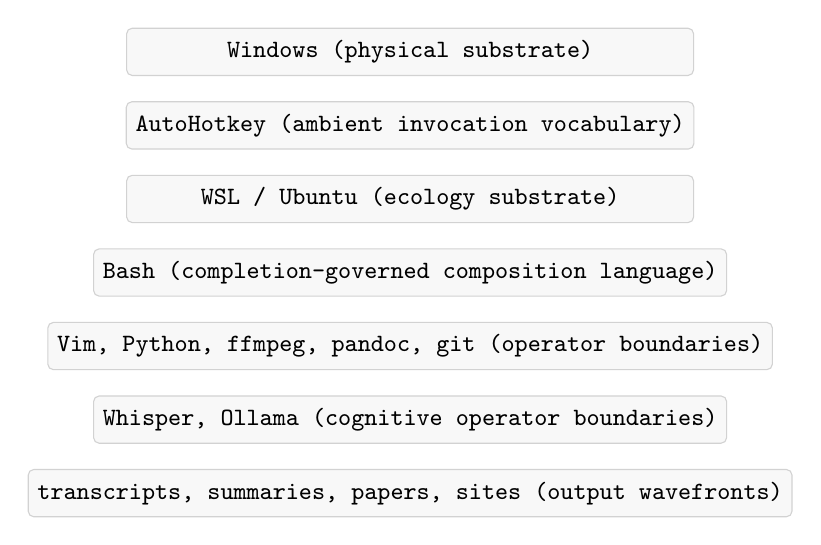
\begin{tikzpicture}[
  node distance=0.32cm,
  box/.style={
    draw, rounded corners=2pt,
    minimum width=7.2cm, minimum height=0.6cm,
    font=\small\ttfamily, align=center,
    fill=codebg, draw=codeframe,
  }
]
\node[box] (win)   {Windows (physical substrate)};
\node[box] (ahk)   [below=of win]   {AutoHotkey (ambient invocation vocabulary)};
\node[box] (wsl)   [below=of ahk]   {WSL / Ubuntu (ecology substrate)};
\node[box] (bash)  [below=of wsl]   {Bash (completion-governed composition language)};
\node[box] (ops)   [below=of bash]  {Vim, Python, ffmpeg, pandoc, git (operator boundaries)};
\node[box] (cog)   [below=of ops]   {Whisper, Ollama (cognitive operator boundaries)};
\node[box] (out)   [below=of cog]   {transcripts, summaries, papers, sites (output wavefronts)};
\end{tikzpicture}
\end{center}

Each layer is not a collection of applications to visit. It is a
collection of behavior boundaries available for invocation. The ecology
does not execute in sequence. It flows: each stage becomes active when
its prerequisite completions arrive, signals its own completion, and
passes the wavefront downstream.

\subsection{AutoHotkey: Ambient Invocation}

AutoHotkey is typically described as a keyboard macro tool. In a flow
computing context it is an \emph{ambient invocation vocabulary}: a
layer of named completion-governed process activations that can be
triggered from any window state, without a terminal context switch.

Each hotkey in a flow-oriented AutoHotkey configuration is not a
shortcut to a GUI destination. It is a \emph{named completion trigger}:
it activates a process network whose internal stages are governed by
their own completion relationships. The hotkey fires the first
wavefront; the downstream stages fire themselves.

The accumulated hotstring vocabulary is equally significant. Hotstrings
are not abbreviations. They are \emph{domain-specific invocation tokens}:
compressed names for recurring process expressions in the user's
specific knowledge domain. The vocabulary crystallizes through use,
each entry marking a completion relationship that has proved stable
and general enough to name.

Reading a mature AutoHotkey file is not reading a configuration
document. It is reading a partial specification of a process ecology:
a record of which invocation relationships the user has stabilized
into named tokens.

\subsection{The Principle of Earned Automation}

A widespread misunderstanding of automation holds that any repetitive
task should be automated as quickly as possible. This view treats
automation as a primary goal and measures productivity by the density
of scripts and shortcuts accumulated.

Flow computing suggests a different principle: \emph{do not automate
a process until its completion relationships have stabilized}.

A process whose structure is still being discovered cannot be
meaningfully automated. Premature automation does not eliminate the
missing mathematician; it merely hardens the confusion into software.
The scripts break. The shortcuts become obsolete. The automation
requires more coordination overhead than the manual process it
replaced.

The purpose of performing a process manually is not inefficiency.
It is \emph{observation}. Repetition reveals the actual boundaries
of the process: the representations that move between stages, the
failure modes, the edge cases, and the completion conditions that
genuinely govern successful execution. Only when these relationships
become stable---when the process reliably produces the same
completion event from the same prerequisites---does automation
become appropriate.

Automation is therefore not the beginning of process understanding
but its \emph{consequence}. The ecology grows not by aggressively
scripting every task but by waiting until each process has disclosed
its own structure, and then naming it.

\subsection{From Repetition to Naming}

The transition from manual process to automated process occurs
through a recognizable sequence: a workflow first exists as a
sequence of manually executed actions; after sufficient repetition,
the sequence becomes recognizable as a coherent unit with stable
boundaries; the unit receives a name; the name becomes a shell
function, a script, an alias, or an AutoHotkey invocation.

The process has been compressed into a symbol. But what makes
the compression valid is not frequency of recurrence alone. It is
that the completion relationships have been understood. The name
is a referential expression---in Fant's sense---that maps to an
autonomous process expression whose behavior is already known.

A concrete example: the sequence

\begin{lstlisting}
yt-dlp "$URL" -x --audio-format mp3 -o audio.mp3
whisper audio.mp3 --output_format txt
ollama run mistral "Summarize:" < audio.txt > summary.txt
pandoc summary.txt -o summary.html
\end{lstlisting}

becomes, after sufficient manual repetition and structural
understanding, a single named invocation: \texttt{overview}.

The name does not replace the process. It refers to a process
expression whose internal completion relationships are already
understood. Naming is \emph{referential compression of earned
understanding}.

\subsection{AutoHotkey as a Fossil Record of Process Discovery}

An AutoHotkey configuration file, viewed through the lens of earned
automation, is a \emph{fossil record of process stabilization}: a
historical record of which processes, in the ecology's development,
reached the threshold of stable completion relationships and received
names.

Each hotkey marks a process that proved sufficiently recurrent,
sufficiently well-understood, and sufficiently stable to deserve a
dedicated invocation. Each hotstring marks a concept, transformation,
or expression pattern that recurred with sufficient frequency and
stability to deserve compression.

The density of entries in a mature AutoHotkey file is not a measure
of productivity obsession or shortcut accumulation. It is a measure
of how many completion relationships have been discovered, observed,
and stabilized over the history of the user's work. The file
accumulates like geological strata: each layer marking a period in
which certain process structures became understood.

A mature AutoHotkey file is therefore neither a configuration file
nor a shortcut collection. It is a partial map of the process
ecology's evolution---a record not of what the user does, but of
what the user has \emph{come to understand well enough to name}.

\subsection{Why Most Automation Fails}

Most automation efforts fail because they attempt to automate
\emph{tasks} rather than \emph{processes}. Tasks are surface
manifestations: the visible actions a person performs. Processes
are underlying structures: the completion relationships that
govern why those actions occur in a particular order and what
representations move between them.

When the underlying process structure is still changing---when
the completion relationships are not yet stable---automating the
surface task produces a script that encodes the current confusion.
The script breaks as the process evolves. The maintenance burden
exceeds the automation benefit. The missing mathematician has not
been eliminated; she has been replaced by a brittle script that
requires constant repair.

The flow computing approach delays automation until the process
has disclosed its structure. This produces fewer automations, but
the automations that survive become durable operator boundaries:
behavior boundaries that compose reliably with other boundaries,
signal completion predictably, and participate in larger
process networks without requiring continuous maintenance.

The goal is not maximum automation. The goal is \emph{stable
invocation}: a vocabulary of named process expressions whose
completion relationships are understood, whose behavior is
trustworthy, and whose composition produces process ecologies
that coordinate themselves.

\subsection{Vim Macros as Deferred Process Crystallization}

Vim macros occupy a theoretically interesting position between
manual execution and permanent automation. A macro records a
sequence of transformations into a named register and allows that
sequence to be replayed without yet elevating it to the status of
a permanent named process expression.

The typical progression in a flow computing ecology is:

\[
\text{manual execution}
\;\to\;
\text{macro}
\;\to\;
\text{script}
\;\to\;
\text{named invocation}
\]

Recording a transformation sequence into register \texttt{q}:

\begin{lstlisting}
qq        " begin recording into register q
...       " perform the transformation sequence
q         " stop recording
\end{lstlisting}

and then executing it at increasing scale:

\begin{lstlisting}
@q        " execute once: observe the result
100@@     " execute 100 times: test at scale
10000@@   " execute 10000 times: commit to the transformation
\end{lstlisting}

is a laboratory for process discovery. The macro occupies the
boundary between observation and automation: the transformation
is sufficiently understood to be repeatable, but not yet stable
enough to deserve referential compression into a permanent name.

In Fant's terms, a macro is a \emph{provisional process
expression}: an autonomous expression that has been transcribed
but not yet promoted to referential status. It can be invoked
repeatedly to test whether its completion relationships are
genuinely stable---whether the same input consistently produces
the same completion event---before the cost of permanent naming
is incurred.

The macro therefore serves the principle of earned automation
not by automating the discovered process but by providing a
low-cost instrument for observing it at scale. The practitioner
applies the macro a hundred times, or ten thousand times, and
watches. If the completion relationships hold under repetition,
the macro earns promotion. If they fail---if edge cases appear,
if the transformation breaks on certain inputs---the provisional
expression is revised before it is crystallized.

A Vim macro is therefore not merely a recorded keystroke sequence.
It is a \emph{temporary behavioral scope}: a bounded container
for process structure that can be invoked repeatedly before being
promoted to a textual process expression. The macro register
(\texttt{q}, \texttt{a}, \texttt{b}, \ldots) is the scope's
name. The recorded content is its autonomous expression. The
repeated invocation (\texttt{100@@}) is stress-testing under
repeated wavefront propagation.

In this sense, macros occupy the same ecological niche as shell
functions in Bash: both are provisional containers for process
structure undergoing validation. The difference is form: the
shell function is a textual definition; the macro is a recorded
behavioral trace. Both are incomplete process expressions in
Fant's sense---referential shorthands awaiting the moment of
sufficient stability to deserve permanent names.

\subsection{Tab Completion as Ecological Sensing}

Tab completion is conventionally described as a typing convenience:
the shell expands a partial filename or command name to its full
form. Within a flow computing ecology it serves a structurally
deeper role: it is a form of \emph{environmental sensing}.

Before invoking a process that produces a representation, the
flow-literate practitioner habitually asks whether that
representation already exists:

\begin{lstlisting}
overview<TAB>        # does overview.txt or overview.html exist?
transcript<TAB>      # has this audio already been transcribed?
summary<TAB>         # has this document already been summarized?
\end{lstlisting}

The tab completion mechanism reveals the current completion state
of the ecology. Which wavefronts have already propagated? Which
process boundaries have already been crossed? Which residues are
already available for downstream invocation?

The same sensing function is performed by shell history recall
(\texttt{Ctrl-R}: has this pipeline been run before, and with
what arguments?), by file globbing (\texttt{ls *summary*}: what
summaries currently exist in this scope?), and by AutoHotkey's
own recognition of previously typed hotstrings (has this
invocation token already been defined?).

These mechanisms share a common logic: \emph{discover before
produce}. A new wavefront should be generated only after the
practitioner has determined that no adequate wavefront already
exists. In a GUI environment, this determination is difficult
because intermediate representations are hidden inside
applications. In a flow computing ecology, the filesystem is
a transparent archive of captured wavefronts, and the shell's
completion and history mechanisms are instruments for consulting
that archive before committing to new computation.

This is not merely a practical efficiency. It reflects a
theoretical property of the ecology: residue is reusable.
A captured wavefront does not expire. If \texttt{transcript.txt}
exists and is complete, the transcription process need not run
again. The completion event that produced it is already in the
ecology's memory, available for any downstream invocation that
requires it. Tab completion is the practitioner's primary
instrument for reading that memory before writing to it.

The significance of a mature AutoHotkey configuration is not that
it contains shortcuts. A desktop operating system already provides
shortcuts. The significance is that a flow-oriented AutoHotkey
vocabulary develops into a \emph{personal invocation language}:
a command language for process activation rather than a menu system
for software navigation.

Many entries in such a vocabulary no longer correspond to application
launches at all. They correspond to process expressions:
\textit{download-and-transcribe}, \textit{summarize-corpus},
\textit{convert-document}, \textit{normalize-text},
\textit{generate-overview}, \textit{publish-site}. Each token
is a referential expression for a larger completion-governed process
network. When the user invokes it, they are not selecting a
destination. They are naming a desired transformation and delegating
its coordination to the structure of the process expression that the
name encodes.

The resulting vocabulary has the structure of a language whose
lexical items are not nouns but \emph{verbs of process activation}.
This is the precise inversion of the application model, in which
the vocabulary consists of nouns---application names designating
places to visit. In the invocation language, no place is visited.
A transformation is named, and the wavefront is released.

This distinction matters beyond terminology. An application
vocabulary grows by accumulating software. An invocation vocabulary
grows by accumulating \emph{understood processes}. The first
measures the user's access to tools. The second measures the user's
comprehension of their work at the level of completion relationships.
A user with a rich invocation language has done the cognitive work
of understanding which transformations recur in their domain,
what representations move between stages, and where the genuine
completion boundaries lie. The language is an artifact of that
understanding.

\subsection{Bash: The Completion-Governed Composition Language}

Bash is the composition language of the ecology. Its primary data type
is the stream. Its primary operators encode completion relationships
directly:

\begin{itemize}
\item \texttt{|} couples two behavior boundaries, passing the output
  wavefront of the first to the input of the second.
\item \texttt{\&\&} invokes the second process only when the first
  signals success (exit code 0)---a logical completion condition.
\item \texttt{||} invokes the second only when the first signals
  failure---the NULL wavefront case.
\item \texttt{>} and \texttt{<} route wavefronts to and from
  persistent named representations (files).
\item The \texttt{for} loop iterates a process boundary over a
  collection, each iteration governed by the same completion
  relationships.
\end{itemize}

A knowledge-work pipeline in Bash:

\begin{lstlisting}
for f in *.mp3; do
  base="${f%.mp3}"
  whisper "$f" --output_format txt -o "${base}.txt" \
    && ollama run mistral "Summarize concisely:" \
         < "${base}.txt" > "${base}_summary.txt"
done
cat *_summary.txt \
  | ollama run mistral "Synthesize these summaries:" \
  > overview.txt \
  && pandoc overview.txt -o overview.html \
  && git add overview.html && git commit -m "auto: overview"
\end{lstlisting}

Every \texttt{\&\&} in this pipeline is a completion gate: the next
stage fires only when the previous stage's output is complete and
correct. The pipeline does not advance because a clock ticked. It
advances because the logic of completion relationships determines that
it should.

\subsection{The Full Knowledge Wavefront}

The complete knowledge pipeline traces a wavefront from raw source
to published product through a succession of completion-governed
invocations:

\[
\underbrace{\texttt{yt-dlp}}_{\substack{\text{acquire}\\\text{(URL complete)}}}
\;\to\;
\underbrace{\texttt{whisper}}_{\substack{\text{transcribe}\\\text{(audio complete)}}}
\;\to\;
\underbrace{\texttt{ollama}}_{\substack{\text{summarize}\\\text{(text complete)}}}
\;\to\;
\underbrace{\texttt{ollama}}_{\substack{\text{synthesize}\\\text{(summaries complete)}}}
\;\to\;
\underbrace{\texttt{pandoc}}_{\substack{\text{format}\\\text{(overview complete)}}}
\;\to\;
\underbrace{\texttt{git}}_{\substack{\text{version}\\\text{(html complete)}}}
\]

Each arrow is a completion event: the downstream stage is invoked
not by a scheduler but by the logical fact that its prerequisites
are satisfied. The intermediate representations---\texttt{.mp3},
\texttt{.txt}, \texttt{\_summary.txt}, \texttt{overview.txt},
\texttt{.html}---are not products. They are wavefronts: intermediate
persistence states that encode the completion of one boundary and
the readiness condition for the next.

The product is not any of these files. The product is the
appreciation of differentness---Fant's phrase for what process
ultimately realizes---that the entire wavefront propagation has
achieved.

\subsection{Persistence as Wavefront Capture}

In a flow computing ecology, files are not primarily storage objects.
They are \emph{captured wavefronts}.

An audio file records the completion of acquisition. A transcript
records the completion of transcription. A summary records the
completion of condensation. An HTML file records the completion of
formatting. Each persistent representation marks the completion
boundary of a particular process and simultaneously constitutes
the invocation condition for subsequent processes. The file exists
at the intersection of two completion events: the completion it
records and the completion it enables.

The filesystem therefore functions as a \emph{memory of completed
wavefronts}. This is not a metaphor. It is a structural description
of what files are in this context. The conventional view treats
files as storage: containers that hold data between uses. The flow
computing view treats files as temporal wavefront markers: evidence
that a process boundary was reached, and readable proof that the
next boundary may be attempted.

This is why a mature flow computing workflow preserves intermediate
representations rather than discarding them after each stage.
\texttt{audio.mp3}, \texttt{transcript.txt}, \texttt{summary.txt},
\texttt{overview.txt}, \texttt{overview.html} are not waste
products of the pipeline. They are the pipeline's memory: a
record of which wavefronts have propagated and a set of
re-invocable starting conditions for any stage that needs to be
rerun, inspected, or rerouted.

This also explains the debuggability of flow computing workflows
that was noted in the Unix section. Because each intermediate
representation is a captured wavefront rather than a hidden internal
state, the entire history of a pipeline execution is visible on
disk. The pipeline can be restarted from any captured wavefront.
A failed downstream stage does not require rerunning the entire
pipeline; it requires only identifying which wavefront is the last
complete one and reinvoking from there.

\subsection{Whisper and Ollama as Cognitive Operator Boundaries}

The integration of Whisper and Ollama into a flow computing ecology
deserves particular attention because it illustrates the power of
treating AI capabilities as completion-governed operator boundaries
rather than as application destinations.

When Ollama is invoked as a GUI application or a web interface,
the user is the mathematician: they decide when to paste in the
input, when to submit the query, when to copy the output. The
language model's cognitive capability is enclosed within an
application that requires external coordination at each use.

When Ollama is invoked as a Bash pipeline stage, the language
model is a \emph{completion-governed behavior boundary}: it receives
an input stream, transforms it, and emits an output stream. It fires
when its input is complete. It signals completion when its output is
stable. The mathematician has been removed. The cognitive capability
is available to the entire ecology, invocable from any stage in any
pipeline, without any GUI visit.

This is not a minor convenience. It is the difference between a
cognitive tool that requires external coordination at every use and
a cognitive operator boundary that participates in completion-governed
process networks as a first-class member of the ecology.

% ============================================================
\section{Personal Languages as Logically Determined Expression Documents}
% ============================================================

Fant distinguishes in \textit{Computer Science Reconsidered} between
\emph{autonomous} and \emph{referential} process expression. An
autonomous expression is complete in itself: it contains all the
coordination behavior necessary for self-realization. A referential
expression uses shorthands and appeals to established conventions,
but must remain mappable to an autonomous expression.

A mature flow computing workflow develops an extensive referential
expression vocabulary over time: shell aliases, shell functions,
Bash scripts, Python utilities, AutoHotkey hotstrings, Makefile
targets. Each entry in this vocabulary is a referential expression:
a named shorthand, mappable to the underlying network of completion
relationships that it abbreviates.

This accumulated vocabulary is not a configuration file. It is a
\emph{logically determined expression document}: a record of which
completion-governed processes have been found stable enough, general
enough, and recurrent enough to deserve names.

The vocabulary grows through a recognizable logic. A pipeline that is
first written inline becomes a shell function when it proves
recurrent. A shell function that is called frequently becomes an
alias. An alias that needs to be accessible from any context becomes
an AutoHotkey hotstring. Each step in this progression is a step
toward greater referential compression of an increasingly well-
understood completion relationship.

Reading a mature expression document reveals the user's process
ecology at the level of its logical structure. Every entry is a
completion relationship that has stabilized. Every name is a
wavefront that has been given a token. The document is, in Fant's
terms, a specification of the spontaneous behavior of the ecology:
a map of which completions invoke which processes.

Crucially, the document is readable, inspectable, and modifiable in
a way that an application's internal logic never is. The referential
expression is transparent to the completion relationships it
encodes. There is no hidden mathematician inside the vocabulary.
The coordination behavior is explicit.

% ============================================================
\section{Computational Literacy as Completion Fluency}
% ============================================================

The conventional account of computational literacy identifies it with
proficiency in the use of applications. A computationally literate
person can use word processors, spreadsheets, email clients, and
browsers. More advanced literacy might include some programming
knowledge.

The flow computing paradigm implies a different account. Literacy is
not proficiency in operating external coordinators. Literacy is
fluency in reading and writing completion-governed process networks:
knowing which operator boundaries are available in an ecology, what
representations each speaks, what completion event each signals, and
how they compose into larger expressions.

This is, precisely, fluency in a logically determined system. The
flow-literate practitioner understands the ecology neighborhood by
neighborhood, in humanly graspable steps, exactly as Fant describes
building trust in a logically determined circuit. She does not need
to maintain a global state model. She needs to understand local
completion relationships and compose them into larger expressions.

Such literacy is more fundamental than conventional programming
literacy in the following sense: programming literacy asks whether
you can express an algorithm in a notation a machine can execute;
flow literacy asks whether you can express a completion-governed
process network in terms that are self-coordinating. The second
question is closer to the actual subject of computer science as Fant
defines it: the science of process expression, not the science of
computation.

It is also more achievable for most practitioners. The operator
boundaries of a Unix ecology are largely provided. Whisper, Ollama,
Pandoc, Git, and the standard Unix toolchain are already complete,
well-specified behavior boundaries. Flow literacy requires knowing
them, understanding their completion events, and composing them.
The sophistication is in the composition; the implementation of the
individual boundaries has already been done.

% ============================================================
\section{Modal Computation and Nested Scope: Vim, Byobu, and Spherepop}
% ============================================================

The flow computing paradigm, as developed so far, concerns
process composition: how operator boundaries are coupled by
completion relationships and how wavefronts propagate through
networks of invocations. But Fant's deeper principle---that
coordination should be \emph{local, compositional, and explicit}
rather than imposed from outside---extends beyond process
composition into the structure of the computational environment
itself.

Unix pipes express this principle at the level of processes.
Vim expresses it at the level of interaction. Byobu expresses
it at the level of workspace organization. And underneath all
three, at the level of formal semantics, the same structure
appears in the Spherepop calculus of nested irreversible scopes.

\subsection{Vim as Modal Computation}

Most text editors are application-centric. The user enters text;
the editor provides commands; the commands are secondary
affordances of a predominantly passive interface. The editor is
a place. Commands are decorations on it.

Vim inverts this relationship. The fundamental abstraction of Vim
is not the command but the \emph{mode}. Normal mode, insert mode,
visual mode, command-line mode, operator-pending mode: each mode
defines a local behavioral neighborhood within which particular
transformations are admissible. A key sequence acquires meaning
only relative to the currently active mode. The same keystroke
that inserts a character in insert mode deletes a word in normal
mode or selects a region in visual mode.

This is structurally analogous to a logically determined system.
The active mode is a completeness condition that gates which
transformations may be invoked. A keystroke is a potential name
whose transformation rule is determined by the mode context in
which it is formed. Coordination is local: the current mode is
the minimal context required to determine what any action means.
There is no global application state to consult; the mode
provides all the context the operation requires.

The editor does not manage the user's actions with an external
controller. The mode \emph{is} the controller---but it is a
local, compositional controller, embedded in the expression
rather than imposed from outside. Vim is, in this sense, a
logically determined interaction surface.

\subsection{Operators and Scopes as Compositional Grammar}

Vim extends the local composition principle into the structure
of its commands. Many Vim operations are not atomic actions
but \emph{compositions of independent components}:

\begin{center}
\begin{tabular}{lll}
\textbf{Operator} & \textbf{Motion/Scope} & \textbf{Command} \\
\hline
\texttt{d} (delete) & \texttt{aw} (around word) & \texttt{daw} \\
\texttt{c} (change) & \texttt{i"} (inside quotes) & \texttt{ci"} \\
\texttt{y} (yank)   & \texttt{ap} (around paragraph) & \texttt{yap} \\
\texttt{gq} (format) & \texttt{ip} (inside paragraph) & \texttt{gqip} \\
\end{tabular}
\end{center}

An operator expresses a transformation: delete, change, yank,
format, indent. A motion expresses a scope: character, word,
sentence, paragraph, delimited region. The resulting command is
formed compositionally. The operator is a completion-governed
function waiting for a scope to complete its invocation condition.
The motion is that completion.

This mirrors the Unix pipeline principle precisely. \texttt{daw}
is a two-stage pipeline: a deletion operator coupled to a scope
boundary, the scope boundary forming the completion condition
that invokes the deletion. The operator-pending mode is the
state in which the operator has been named but the scope has
not yet completed: a behavior boundary waiting for its input
wavefront to arrive.

The space of possible commands is not enumerated but generated.
There are perhaps a dozen operators and several dozen motions;
their cross product yields hundreds of compositional commands
that the user can express without having memorized any of them
as atomic operations. Complex editing behavior emerges from
combinations of small, orthogonal components, exactly as complex
pipeline behavior emerges from combinations of simple operator
boundaries. The Unix philosophy is alive inside the keystroke.

\subsection{Vim's Shell Integration as Pipeline Stage}

Vim does not merely resemble a flow computing environment. It
participates in one. The \texttt{:!} command executes an external
process and displays its output. The \texttt{:r~!cmd} command
inserts the output of an external process into the current buffer
as a new wavefront of text. Most significantly, \texttt{:\%!cmd}
pipes the entire buffer through an external process and replaces
it with the result.

In each case, Vim becomes a stage in a pipeline: a behavior
boundary that can receive a wavefront from an upstream process,
present it to a human operator for inspection or modification,
and pass the modified wavefront to a downstream process. The
human is not a mathematician who manages the pipeline from
outside. The human is a cognitive operator boundary embedded
within the pipeline: a stage whose completion event is a
deliberate save or write.

This is how Vim fits into the broader ecology. It is not an
application that exists alongside the pipeline. It is a
pipeline stage that provides a human-readable, modally-structured
transformation surface at any point where human judgment is
required.

\subsection{Byobu as Hierarchical Process Space}

Byobu is a terminal multiplexer: it allows a single terminal
connection to host multiple shell sessions, each divided into
windows and panes. Most users treat it as a convenience for
managing many terminals at once. In a flow computing ecology,
it is something structurally more significant.

Byobu instantiates a \emph{nested scope architecture}: a
hierarchy of behavioral containers, each enclosing the levels
below it and providing a distinct organizational context:

\begin{center}
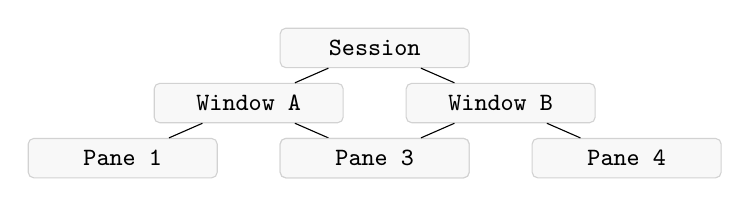
\begin{tikzpicture}[
  level distance=0.7cm,
  sibling distance=3.2cm,
  every node/.style={draw, rounded corners=2pt, font=\small\ttfamily,
    fill=codebg, draw=codeframe, minimum width=2.4cm,
    minimum height=0.5cm, align=center},
]
\node {Session}
  child { node {Window A}
    child { node {Pane 1} }
    child { node {Pane 2} }
  }
  child { node {Window B}
    child { node {Pane 3} }
    child { node {Pane 4} }
  };
\end{tikzpicture}
\end{center}

Each level in this hierarchy is a scope: a bounded context with
its own identity, its own set of active processes, and its own
relationship to the levels that contain it. A pane contains a
shell. A window contains panes organized around a shared task
context. A session contains windows organized around a project.
Sessions can be detached and reattached, persisting across
disconnections: the session is a persistent scope that outlives
any particular terminal instance.

This is the flow computing principle of local coordination
applied to workspace organization. Each scope is coherent on
its own terms. Processes inside a scope inherit its context
without needing to reach outside it for coordination. The
scope is self-sufficient: it contains the environment, history,
aliases, working directory, and active processes that its
inhabitants require.

\subsection{Byobu Keybindings as Scope Navigation}

Byobu's keybinding structure exposes the session-window-pane
hierarchy as a navigable space rather than a flat list of
terminals. The standard bindings directly reflect the nested
scope architecture:

\begin{itemize}
\item \textbf{F2} creates a new window (a new top-level scope
  within the session).
\item \textbf{Shift-F2} subdivides the current window
  horizontally; \textbf{Ctrl-F2} subdivides it vertically.
  Both create new pane-level scopes within the current window.
\item \textbf{Shift-F3} / \textbf{Shift-F4} move focus between
  sibling panes: lateral navigation within a scope level.
\item \textbf{F3} / \textbf{F4} move between windows:
  navigation at the enclosing scope level.
\item \textbf{F6} detaches the entire session, preserving all
  scope state while freeing the terminal connection.
  \textbf{Shift-F6} detaches without logging out.
\item \textbf{Alt-PgUp} / \textbf{Alt-PgDn} enter scrollback
  mode: access to up to 10,000 lines of a pane's wavefront
  history, navigable and copyable without disrupting the active
  process.
\item \textbf{Ctrl-a~\textasciitilde} saves the current window's
  scrollback buffer: explicitly capturing the pane's residue
  as a persistent file.
\end{itemize}

The practitioner navigating this hierarchy is not selecting
terminals. They are moving between scopes. Each scope has a
semantics: this window is the transcription workspace; that
window is the editing workspace; this pane runs the Python
server; that pane runs the build loop. The scopes are
persistent---they survive connection interruptions, system
sleep, and context switches to other work. Reattaching a Byobu
session is not opening a terminal. It is re-entering a process
ecology that has been running in your absence, its wavefronts
propagating, its residue accumulating.

The scrollback buffer deserves particular note. Each pane
maintains up to 10,000 lines of output history: the full
residue of every process that has run within that scope.
This residue is inspectable (\textbf{Alt-PgUp}), copyable,
and saveable (\textbf{Ctrl-a~\textasciitilde}). The pane is
not merely a process container. It is a bounded scope with a
memory of its own completed wavefronts.

\subsection{Development as Wavefront Refinement}

The flow computing character of a software development workflow
is most clearly visible in the iterative edit-run cycle. A
typical configuration binds:

\begin{itemize}
\item \textbf{Alt-F9}: open the active script in Vim for
  editing.
\item \textbf{F8}: execute the script and observe its output
  in an adjacent pane.
\end{itemize}

The resulting cycle is a completion-governed feedback loop:

\[
\underbrace{\text{edit}}_{\substack{\text{modify expression}\\\text{(judgment complete)}}}
\;\xrightarrow{\text{Alt-F9 / :w}}\;
\underbrace{\text{save}}_{\substack{\text{capture wavefront}\\\text{(edit complete)}}}
\;\xrightarrow{\text{F8}}\;
\underbrace{\text{execute}}_{\substack{\text{run process}\\\text{(script complete)}}}
\;\xrightarrow{}\;
\underbrace{\text{residue}}_{\substack{\text{observe output}\\\text{(run complete)}}}
\;\xrightarrow{}\;
\underbrace{\text{revise}}_{\substack{\text{judgment invoked}\\\text{(residue complete)}}}
\]

Each arrow is a completion event. The save completes the edit.
The F8 invocation completes because the file exists and is
valid. The execution completes and deposits its output as
residue in the adjacent pane. The observation of the residue
completes the cognitive evaluation, which either terminates
the cycle (the output is correct) or invokes a new edit
pass (the output reveals a fault).

This is precisely the second-order flow computing model:
a feedback cycle realized as a series of discrete
completion-governed wavefronts. Each iteration is a complete
feed-forward pass. The cycle is not a continuously active
control loop. It is a sequence of invocations, each triggered
by the completion of the previous one.

The same structure governs web development in a Byobu
multi-pane layout. One pane edits HTML and JavaScript in Vim.
An adjacent pane runs a local Python HTTP server:

\begin{lstlisting}
python3 -m http.server 8000
\end{lstlisting}

A third pane (or a browser window) inspects the served output.
The three panes are three behavior boundaries in a
completion-governed loop: edit completes, server serves the
new wavefront, browser renders the residue, observation
invokes the next edit. No application manages this loop.
No scheduler coordinates the panes. The structure of the
Byobu workspace, the scope each pane occupies, and the
completion event of each process \emph{are} the coordination.

The ecology manages itself.

Each shell session is a bounded computational scope. It
possesses its own environment variables, command history,
working directory, alias and function definitions, and set
of active processes. A child shell inherits from its parent
but modifies only its own copy of the inherited state. When
the child exits, its modifications are gone. The parent is
unchanged.

This scoping behavior is not a technical detail. It is the
same organizational principle that runs through the entire
flow computing ecology: local coherence, explicit inheritance,
no hidden global state that requires external coordination.
The shell session is a self-contained behavior boundary. Its
completion event is the shell's exit. Its residue is whatever
it has written to the shared filesystem before exiting.

The hierarchy of Byobu scopes---pane, window, session---is
therefore a hierarchy of nested behavior boundaries, each
self-coordinating within its local context, each capable of
composing with neighboring scopes through the shared filesystem
and process namespace.

\subsection{Nested Scopes and Spherepop}

The Spherepop calculus, developed as a formal model of
irreversible event sequences, describes computation as the
progressive resolution of nested semantic bubbles. A bubble
is a bounded scope that can contain sub-bubbles. When a
bubble resolves---reaches its completion event---it either
pops (irreversibly commits its result to the enclosing scope)
or collapses (discards its contents without effect). The
enclosing scope receives the result or the absence of a result,
and its own resolution proceeds accordingly.

The structural parallel with the Byobu/shell/Vim hierarchy is
precise. A pane is a bubble. Its completion event is the
process that exits within it. When the process completes, the
result---the wavefront it has written to the filesystem or
piped to a sibling---propagates to the enclosing scope. The
window is a larger bubble: its completion is the coherent
resolution of its constituent panes around a shared task. The
session is a larger bubble still.

The analogy extends to Vim's modal structure. Each Vim mode is
a local scope: a bounded behavioral context within which
particular transformations are admissible. The mode transition
is not an application-level state change; it is a scope
transition. Entering operator-pending mode is entering a
sub-bubble that waits for a motion to complete its invocation
condition. When the motion arrives, the sub-bubble resolves:
the operator fires, the text is transformed, the mode returns
to normal.

In Spherepop's terms: operator-pending mode is an open bubble
whose resolution condition is the receipt of a valid motion.
The motion is the event that pops the bubble. The transformation
is the result deposited in the enclosing scope.

\subsection{Scope Before Process}

Traditional operating system descriptions emphasize processes
as primary entities and scopes---directories, sessions,
namespaces---as secondary organizational containers. The process
is the unit of computation; the scope is merely where it runs.

The lived experience of a mature Unix flow computing environment
inverts this relationship. The practitioner navigates sessions,
windows, panes, projects, directories, and modal editing
surfaces. Processes appear within these scopes and inherit
their context. The question the practitioner asks is not
\emph{which process am I running?} but \emph{which scope am I in?}

The scope comes first. The process is an inhabitant of the scope.

This inversion is not merely phenomenological. It has structural
consequences. When scope is primary, the computational environment
becomes navigable as a space of nested contexts rather than a
flat list of running programs. The practitioner can orient
themselves by scope membership rather than by process identity.
They can carry context from one process invocation to the next
by remaining within the same scope. They can isolate experimental
work in a new scope without affecting established contexts. They
can close a scope when its work is done and trust that its
residue---whatever it has deposited in the shared filesystem---
is available to other scopes that need it.

This is the deepest sense in which flow computing is not merely
about pipes. Unix is not merely a philosophy of processes. It
is a philosophy of \emph{nested scopes within which processes
become meaningful}: scopes that provide local coordination,
local context, and local completion boundaries, composing into
larger scopes through the universal medium of the shared
filesystem and the universal representation of the text stream.

Vim's modes, Byobu's session-window-pane hierarchy, and
Spherepop's nested bubbles are three expressions of the same
underlying principle: that coordination should be local,
compositional, and explicit; that the boundaries of a scope
should determine what is admissible within it; and that the
completion of a scope should deposit its residue in the
enclosing scope rather than requiring an external coordinator
to collect and route it.

\subsection{The Recurrence of Nested Completion Structures}

What becomes visible across the full ecology is not merely
that each tool embodies the flow computing principle, but that
the same organizational pattern recurs at every scale. Operator
boundaries compose into commands. Commands compose into scripts.
Scripts compose into pipelines. Pipelines inhabit panes. Panes
inhabit windows. Windows inhabit sessions. Sessions inhabit
projects. The computational environment exhibits a
\emph{recursive nesting of completion-governed scopes} whose
structure is approximately self-similar across levels of
abstraction:

\begin{center}
\begin{tabular}{ll}
\textbf{Scale} & \textbf{Completion-governed scope} \\
\hline
Keystroke & Vim operator + motion $\to$ command \\
Command & Behavior boundary (stdin $\to$ stdout $\to$ EOF) \\
Pipeline & Coupled behavior boundary chain \\
Pane & Shell session + scrollback residue \\
Window & Task-coherent pane collection \\
Session & Project-coherent window collection \\
Ecology & Named invocation vocabulary \\
\end{tabular}
\end{center}

This self-similarity is not incidental. It is the consequence
of applying a single organizational principle---local
completion-governed coordination---consistently at every level
of the environment's design. Fant discovers the principle at
the level of logic gates. McIlroy encodes it at the level of
processes. Vim expresses it at the level of interaction. Byobu
expresses it at the level of workspace. Spherepop formalizes
it at the level of irreversible event calculus.

The same invariant, reproduced at each scale: a bounded scope
becomes active when its prerequisites are complete, does its
work, signals completion, and deposits its residue in the
enclosing scope. This is the structural claim of the essay,
stated as concisely as possible.

\subsection{The Residue Hierarchy}

The various residue-preserving mechanisms of the ecology form
a natural hierarchy ordered by persistence and commitment:

\begin{center}
\begin{tabular}{lll}
\textbf{Level} & \textbf{Mechanism} & \textbf{Character} \\
\hline
Transient & Pane scrollback buffer & Ephemeral; up to 10k lines \\
Volatile & Shell variable, Vim register & Scope-local; lost on exit \\
Session & Shell history (\texttt{.bash\_history}) & Persistent across sessions \\
Named & Alias, shell function & Referential; explicitly authored \\
Committed & File on filesystem & Captured wavefront \\
Versioned & Git commit & Timestamped residue with provenance \\
Invocable & Script, AutoHotkey entry & Autonomous process expression \\
\end{tabular}
\end{center}

Each level represents a greater degree of commitment to the
stability of the captured wavefront. The progression is not
merely technical; it mirrors the epistemological arc of earned
automation:

\[
\text{observation}
\;\to\;
\text{capture}
\;\to\;
\text{stabilization}
\;\to\;
\text{naming}
\;\to\;
\text{invocation}
\]

A process first produces residue in the most transient form:
output visible in the scrollback buffer, a Vim register holding
an intermediate value. If the output proves useful it is
promoted: written to a file, added to history, crystallized
into a function. If the function proves stable and general
it is promoted further: committed to a script, entered into
the AutoHotkey vocabulary, made invocable from any context.

The AutoHotkey file, the \texttt{.bashrc}, the \texttt{.vimrc},
the Git repository, and the filesystem are therefore not separate
tools with separate purposes. They are successive commitment
levels in a single residue hierarchy: each level encoding
greater confidence that the captured wavefront represents a
genuine completion event in a stable completion-governed process.

% ============================================================
\section{Feedback, Residue, and Second-Order Flow}
% ============================================================

The flow computing paradigm as described so far applies cleanly to
\emph{feed-forward} process networks: acyclic chains in which a
wavefront propagates from source to product through a succession of
completion-governed stages. Document conversion, media processing,
corpus transcription, deployment pipelines---these are first-order
flow computing, and they present no theoretical difficulty.

But real knowledge work is rarely acyclic. A transcript is
summarized; the summary is critiqued; the critique generates a
revised prompt; the revised prompt produces a new summary. Software
is written; tests reveal failures; failures modify requirements;
modified requirements change the code. Scientific inquiry proceeds
by hypothesis, experiment, anomaly, revision, and new hypothesis.
A cycle has formed.

The question this raises is not merely technical. It is theoretical:
does the appearance of feedback cycles mean that flow computing
requires an external coordinator after all---that cycles reintroduce
the missing mathematician?

\subsection{Feedback as Completion-Governed Wavefronts}

The answer is no, provided that feedback is understood correctly.
The threat of a feedback cycle is the threat of \emph{continuous
control}: a downstream process that continuously modifies the
behavior of an upstream process, producing a system that never
reaches a completion boundary and therefore never settles.

But feedback in a flow computing ecology does not need to be
continuous. It can itself be completion-governed. The cycle becomes
a sequence of discrete wavefront propagations:

\[
\text{Wavefront}_1 \;\to\; \text{completion}_1 \;\to\;
\text{feedback wavefront} \;\to\; \text{Wavefront}_2 \;\to\;
\text{completion}_2 \;\to\; \text{feedback wavefront} \;\to\; \cdots
\]

Each iteration of the cycle is a complete feed-forward propagation
that reaches a genuine completion boundary before the next iteration
begins. The cycle is not continuously active. It is a succession of
discrete completion-governed invocations whose structure happens to
include a return path.

In practice, this is precisely what a Bash loop with
\texttt{\&\&} gates is: a sequence of completion-governed wavefronts
in which each iteration's output may condition the next iteration's
input, but no iteration begins until the previous one has signaled
completion. The recursion is real. The missing mathematician is not.

\subsection{Residue: The Memory of Completed Wavefronts}

Every process leaves something behind. This is not a side effect
to be minimized. It is a structural property of completion-governed
process networks that has a name: \emph{residue}.

A transcript is the residue of a transcription process. A summary
is the residue of a condensation process. A critique is the residue
of an evaluation process. A Git commit is the residue of a
versioning process. Residue is what a process deposits at its
completion boundary: the captured wavefront that marks the process
as done and simultaneously constitutes an invocation condition
for future processes.

The concept of residue is what distinguishes memory from mere
storage in a flow computing ecology. A file is storage when it is
an inert container. A file is residue when it is the deposited
completion record of a process whose structure is understood and
whose output forms the prerequisite of a subsequent invocation.

Residue accumulates. As the ecology runs---cycling through
acquisition, transcription, summarization, critique, revision,
publication---a growing corpus of captured wavefronts accumulates
in the filesystem. This corpus is not a database. It is not an
archive. It is the \emph{memory of the ecology}: a record of which
processes have run, what they produced, and what conditions now
exist for future invocation.

In a feedback cycle, residue plays a specific role: the completion
of one pass through the cycle deposits residue that becomes the
prerequisite condition for the next pass. The cycle is
\emph{logically determined by its own accumulating residue}.
The feedback is not continuous control; it is completion-governed
sequential invocation conditioned by the ecology's own memory.

\subsection{Two Regimes of Flow Computing}

This suggests a natural distinction between two regimes:

\textbf{First-order flow computing} describes acyclic completion
networks. A wavefront propagates from source to product through
a fixed topology:
\[A \to B \to C \to D\]
Document conversion, media transcription, corpus formatting,
and deployment pipelines are paradigmatic examples. The completion
relationships are fixed; the wavefront moves in one direction;
the process terminates.

\textbf{Second-order flow computing} describes completion networks
whose topology evolves through the accumulation of residue. A
wavefront propagates through the network; residue is deposited;
the residue modifies the invocation conditions for future
wavefronts; the topology of available invocations changes:
\[A \to B \to C \to \text{residue} \to A'\]
where $A'$ is an invocation of $A$ conditioned on what $C$
deposited. Software development, scientific inquiry, AI-assisted
writing, and organizational learning are paradigmatic examples.
The completion relationships evolve; the wavefront cycles; the
process is potentially unbounded.

The critical observation is that second-order flow computing does
not abandon the flow paradigm. It extends it. The ecology remains
organized around completion-governed invocation; residue provides
the memory that allows invocation conditions to evolve; feedback
cycles become series of discrete wavefront propagations rather than
continuous control processes. The missing mathematician does not
return.

\subsection{The Mechanism: Residue as a Modifier of Invocation
Conditions}

The distinction between first- and second-order flow computing is
not merely that the second involves a loop while the first does
not; Section~7.1 already showed that a loop, properly understood,
is a sequence of discrete completion-governed invocations rather
than a return of continuous control. The real distinction is
structural: in first-order flow computing, the invocation
conditions themselves---which process fires next, and on what
input---are fixed in advance by the topology of the pipeline. In
second-order flow computing, the invocation conditions are
themselves a function of accumulated residue, and can therefore
change from one pass through the cycle to the next.

This is easiest to see by contrasting a static branch with a
residue-conditioned one. A static branch is still first-order flow
computing, even though it involves a conditional:
\[
A \to B \to
\begin{cases}
C & \text{if exit}(B) = 0 \\
D & \text{otherwise}
\end{cases}
\]
The condition here is a fixed property of the topology---it was
written into the pipeline once, by a human or a script, and does
not change as the pipeline runs repeatedly. Second-order flow
computing instead makes the condition itself a residue-dependent
quantity:
\[
A \to B \to C \to \text{residue}_n \to \big(\text{route}(\text{residue}_n) : A \to \{B, B', B''\}\big)
\]
Here the invocation that fires on the next pass---which variant of
$B$ is invoked, or with what parameters---is not fixed by the
pipeline's author but determined by inspecting what has
accumulated. The topology of the network, in other words, is
itself part of what evolves under completion-governed dynamics,
rather than being external to them.

Consider a concrete instance from software engineering: a
continuous-integration harness that, on a test failure, does not
simply report the failure but consults a residue store of prior
bug reports and their eventual resolutions. If the failure's
signature (stack trace, affected module, failing assertion)
resembles a past incident whose residue shows it was resolved by
a particular engineer or a particular class of fix, the harness
routes the failure report to that engineer, or applies a
previously successful automated patch pattern, rather than
following a single static escalation path. The invocation
path---who or what gets invoked next---is determined by the
accumulated residue of prior completions, not by a rule written
once at pipeline-construction time. Nothing in this arrangement
requires a central controller watching the whole history; the
routing decision is a local completion-governed process, applied
each time a new failure wavefront arrives, that happens to consult
memory rather than a fixed table.

The same mechanism appears, at different timescales, across the
domains this essay has already touched on. In scientific inquiry,
an anomalous experimental result (residue) does not merely
terminate the current experiment; it conditions which hypothesis
is tested next, effectively rewriting the topology of the inquiry
process for its next pass. In AI-assisted writing---the regime
most directly relevant to the composition of this essay---a
critique of a draft is residue that conditions not just the
content of the next revision but which \emph{kind} of revision is
attempted: a critique flagging weak evidentiary support routes to
a research-and-citation pass, while a critique flagging unclear
structure routes to a reorganization pass. The critique does not
merely supply new input to a fixed revision function; it selects,
by its content, which revision function is invoked. In
organizational learning, a postmortem document is residue that
conditions which review gates are added to future deployments,
altering the topology of the deployment pipeline itself for
subsequent runs.

In each case, the pattern is the same: a completion event deposits
residue; the residue is inspected, not by an external supervisor
but by the next local invocation in the chain; and the inspection
determines which branch of the process network fires next. This is
what distinguishes second-order flow computing from an ordinary
conditional branch. A conditional branch selects among
pre-specified paths using the current input. Second-order flow
computing selects among paths using the \emph{accumulated history}
of prior completions---and, critically, can grow new paths that
were not anticipated by the original topology, as residue
accumulates in ways the pipeline's original author did not
foresee. The ecology does not merely execute; it learns its own
shape.

\subsection{A Note on Cloud Orchestration}

This analysis has direct implications for how modern distributed
computing architectures should be evaluated. Many enterprise systems
are marketed as event-driven and completion-governed. Yet they
accumulate vast supervisory infrastructure: schedulers,
orchestrators, service meshes, state stores, controller loops.

From the flow computing perspective, this infrastructure is a
collective mathematician. It is external coordination imposed on
a process network that, in principle, could coordinate itself
through local completion relationships. The coordination logic is
not \emph{in} the processes; it is in the supervisory layer above
them.

The question Fant would ask is the right question: why does the
process network require so many external coordinators? A genuinely
flow-computing cloud architecture would attempt to move coordination
into local completion relationships and accumulated residue, reducing
the role of centralized supervisory structures to the minimum the
implementation substrate genuinely requires.

Whether that is fully achievable at internet scale remains open.
What is not open is the diagnosis: centralized orchestrators are
not a feature of scale. They are evidence that the coordination
behavior has not been successfully encoded into the process
network itself.

\subsection{Stochastic Wavefronts and Semantic Admissibility}

The introduction of large language models as cognitive operator
boundaries (Section~6) creates a theoretical complication that
the preceding analysis has deferred. In an NCL circuit or a
deterministic Unix pipeline, the completion criterion is binary
and precise: a data wavefront has either fully propagated or it
has not; the exit code is either zero or nonzero. The wavefront
is either admissible or it is NULL.

A large language model introduces a different regime. The model
accepts a syntactically complete input wavefront and produces a
syntactically complete output. At the shell level, it signals
completion with exit code zero. But the output may be
\emph{semantically inadmissible} for its downstream stage: the
format may be structurally valid but ecologically wrong, the
content may hallucinate a representation that downstream
processes cannot consume, the summary may omit a key claim that
subsequent synthesis depends on.

This is the \emph{weak completion problem}: a cognitive operator
boundary can satisfy syntactic completion while failing semantic
completion. In Fant's terms, it produces a candidate output
that looks like a completed wavefront but is not yet suitable
residue. The downstream stage cannot tell from the shell exit
code alone whether the wavefront it has received is trustworthy.

The solution is a second-order completion criterion:
\emph{admissibility}. Where rigid operator boundaries require
only syntactic completion, cognitive operator boundaries require
that the candidate output pass an admissibility test before
being committed as residue. Formalizing this:

\[
B_i \;\xrightarrow{T_\theta}\; \tilde{B}_{i+1}
\]

where $B_i$ is the input boundary state, $T_\theta$ is a
stochastic cognitive operator, and $\tilde{B}_{i+1}$ is a
\emph{candidate wavefront}---not yet valid residue. The
candidate must satisfy an admissibility functional:

\[
\mathcal{A}\!\left(\tilde{B}_{i+1} \mid C, S, F\right) \;\geq\; \tau
\]

where $C$ is the current context, $S$ is the expected schema,
$F$ is downstream fitness, and $\tau$ is the commitment
threshold. The boundary transition rule becomes:

\[
B_{i+1} =
\begin{cases}
\operatorname{commit}(\tilde{B}_{i+1})
  & \text{if } \mathcal{A} \geq \tau \\[4pt]
\operatorname{repair}(\tilde{B}_{i+1})
  & \text{if } \tau_r \leq \mathcal{A} < \tau \\[4pt]
\operatorname{quarantine}(\tilde{B}_{i+1})
  & \text{if } \tau_q \leq \mathcal{A} < \tau_r \\[4pt]
\operatorname{collapse}(\tilde{B}_{i+1})
  & \text{if } \mathcal{A} < \tau_q
\end{cases}
\]

yielding four possible outcomes: the candidate is committed as
residue; repaired through a corrective loop and reconsidered;
quarantined (preserved but excluded from downstream invocation);
or collapsed (discarded without residue). In practice, this maps
to familiar workflow patterns:

\begin{center}
\begin{tabular}{lll}
\textbf{Outcome} & \textbf{Flow computing meaning} & \textbf{Bash realization} \\
\hline
Commit & Output is valid residue & Write to file, proceed \\
Repair & Retry with revised prompt & Loop with \texttt{\&\&} retry \\
Quarantine & Save for inspection, skip & Write to \texttt{*.suspect/} \\
Collapse & Discard candidate & \texttt{|| rm \$out \&\& exit 1} \\
\end{tabular}
\end{center}

This analysis distinguishes four levels of completion that
a cognitive operator boundary must satisfy:

\begin{enumerate}
\item \textbf{Exit-code completion}: the process exited with
  status 0.
\item \textbf{Format completion}: the output conforms to the
  expected structural representation.
\item \textbf{Semantic completion}: the output contains the
  content that downstream invocations require.
\item \textbf{Ecological completion}: the output is admissible
  as residue in the specific context of the current ecology's
  state.
\end{enumerate}

Only ecological completion constitutes genuine flow completion
in the flow computing sense. A cognitive operator boundary that
achieves only exit-code completion has not yet produced a
wavefront. It has produced a candidate. The admissibility
functional is the gate that converts candidates into residue.

\subsection{The NULL Wavefront as Markov Boundary}

The theoretical significance of Fant's NULL convention extends
beyond the engineering problem of clockless coordination. The
propagating NULL wavefront is, in information-theoretic terms,
a \emph{moving Markov boundary}: a structure that separates
completed computational episodes from each other, creating
conditional independence between them.

Consider an ordinary combinational logic network processing
asynchronously changing inputs. At any given instant, some
gates have propagated their new outputs and others have not.
The network is in an intermediate state. There is no intrinsic
marker distinguishing a completed computation from a partial
one, a stable result from a transient hazard. The boundary
between finished and unfinished is invisible. The network lacks
a natural separator.

NCL's NULL wavefront provides that separator. Every signal
occupies one of two distinguished states: DATA (a computation
is in progress) or NULL (no computation is active). The
alternating cycle:

\[
\text{NULL} \;\to\; \text{DATA} \;\to\; \text{NULL} \;\to\; \text{DATA}
\]

marks the topology of computational episodes. Crossing from
NULL to DATA means: \emph{this computation is now active}.
Crossing back to NULL means: \emph{this computation is
complete}. The NULL manifold is a distinguished surface in
state space. Crossing it is a completion event.

In probabilistic terms: once the NULL wavefront has fully
propagated, everything that was true of the \emph{previous}
computation is irrelevant to the \emph{next} computation. The
NULL state renders the downstream process conditionally
independent of the unresolved internal details of the upstream
process. It is precisely the Markov property: given the
boundary state, past and future are independent.

This connection illuminates the behavior of persistent
intermediate representations in a flow computing ecology.
A captured wavefront file---\texttt{transcript.txt},
\texttt{summary.txt}, \texttt{overview.html}---functions as
a \emph{frozen Markov boundary}. Once the transcript is
complete, the downstream summarization process is
conditionally independent of everything that happened during
audio acquisition and transcription. It does not need to know
about recording conditions, Whisper model versions, audio
quality, or processing time. It needs only the transcript.

The transcript \emph{is} the NULL wavefront, frozen: a
complete, stable separator between the acquisition episode
and the summarization episode. The chain of residue files:

\[
\texttt{audio.mp3} \;\to\; \texttt{transcript.txt} \;\to\;
\texttt{summary.txt} \;\to\; \texttt{overview.txt}
\]

is a chain of Markov boundaries. Each completed artifact
renders the downstream stage conditionally independent of the
internal details of the upstream stage. The stages can be
replaced, updated, or rerun independently without invalidating
the others---provided each replacement produces an output
admissible as the same Markov boundary.

This is why Fant's NCL feels, in retrospect, less like a
hardware design technique and more like a general theory of
computational boundaries. The NULL wavefront is not a trick
for avoiding clocks. It is an explicit mechanism for
constructing Markov-like separators between computational
episodes---boundaries that distinguish what must be known
from what can be safely ignored, at every scale from logic
gates to knowledge pipelines.

\subsection{Thermodynamic Computing: A Structurally Related
Development}

Fant developed NCL to solve a problem in digital circuit design:
how to restore expressional completeness to a Boolean logic
network without appeal to an external clock or coordinator. His
solution was to encode coordination in the logic itself, so that
computation proceeds as the propagation of a wavefront rather
than as a sequence of externally scheduled state transitions.
It is worth noting, without overstating the connection, that a
structurally adjacent move has recently been made from an
entirely different direction: not digital logic seeking to
eliminate an external clock, but analog and statistical physics
seeking to eliminate an external error-correction regime.

Reporting on the nascent field of thermodynamic computing, Ball
(2026) describes two architectures that map, at the level of
mathematical structure if not motivation, onto the distinction
this essay draws between state-centered and wavefront-centered
computation.\footnote{Philip Ball, ``Thermodynamic Computers Go
With the (Energy) Flow,'' \textit{Quanta Magazine}, July 15,
2026.} \emph{Equilibrium} thermodynamic computing encodes a
problem into an energy landscape whose minima represent
admissible solutions; the system is released and left to settle,
and the answer is read off once it has relaxed. \emph{Nonequilibrium}
thermodynamic computing instead encodes the computation into a
stochastic trajectory sustained by continuous energy flow, in
which the trajectory itself---not any terminal state---carries
the result. Although developed independently and for different
reasons, this distinction bears a structural resemblance to the
separation this essay draws between admissible configuration
spaces and continuation dynamics: one mode of computation is
characterized by convergence toward a constrained manifold, the
other by computation performed \emph{as} an evolving trajectory
through state space. The resemblance is mathematical, not
conceptual identity; the two research programs do not share a
theoretical vocabulary and should not be read as making the same
claim.

More directly relevant to the wavefront argument is what these
architectures do with noise. A conventional digital gate is
engineered to operate at energies far above the thermal
fluctuations of its environment precisely so that noise cannot
masquerade as a completed signal; the clock exists, in part, to
give transient hazards time to settle before they are sampled.
Thermodynamic computers invert this relationship. Random thermal
fluctuations are not suppressed but used to explore a
configuration space, with the system's own physics performing
part of the computation for free. This is a structurally similar
inversion to the one Fant makes at the logical level---one
concerns noise versus error correction, the other concerns
clocks versus local completion, and the two should be read as
analogous rather than identical---but both replace an external
authority that manages timing or fidelity with a local mechanism
whose proper behavior is a structural consequence of its own
dynamics rather than of supervision. Whitelam's simulated
denoising circuit, which reconstructs a corrupted image by
letting connection strengths relax toward the configuration that
makes the image most likely, resembles a constrained wavefront
relaxing toward a locally admissible configuration: structure
emerging from the settling of a locally governed process rather
than from any global instruction sequence.

Some caution is warranted before extending this further.
Whitelam offers the striking claim that ``nature uses Langevin
computers programmed by evolution''---a much stronger claim than
most physicists would have advanced a few years ago, and one
that Kaneko, in the same article, meets with explicit reservation
about whether it constitutes a genuine explanatory framework for
biological computation or merely a suggestive analogy. This essay
takes no position on that question. What it notes is narrower:
several independent lines of contemporary work---active
inference, diffusion models, analog and neuromorphic hardware,
reservoir computing, morphological computation, and now
thermodynamic computing---share a common intuition that efficient
computation often consists of shaping a dynamical system so that
its own physical evolution performs inference or optimization,
rather than forcing physical substrates to imitate an idealized
sequence of discrete symbolic operations. Although these fields
differ substantially in objectives, assumptions, and mathematical
machinery, many increasingly rely on continuous dynamical
systems, stochastic differential equations, and constrained
energy landscapes as primary computational objects rather than
treating them merely as implementation details beneath discrete
algorithms. None of these fields
are converging on a single formalism, and thermodynamic computing
in particular remains, in its own literature's words, at a stage
comparable to small-scale quantum computing in the 1990s: a proof
of principle rather than a settled architecture. That direction
of the shift is broadly consistent with the direction this essay
has been arguing for: treating physical dynamics as primary and
symbolic computation as one important realization of a more
general process organization, argued here from the vantage point
of a Unix pipeline rather than a resistor-inductor-capacitor
network. That two such different starting points arrive at
structurally similar distinctions is, at minimum, evidence that
the wavefront-over-clock intuition is not an idiosyncrasy of
Fant's circuit design or of this essay's extension of it.

Put plainly: Fant arrives at this principle through asynchronous
logic design; Unix arrives at it through software composition;
thermodynamic computing arrives at it through statistical
mechanics; active inference arrives at it through variational
physics; diffusion models arrive at it through stochastic
dynamics; reservoir computing arrives at it through nonlinear
dynamical systems; morphological computation arrives at it
through biomechanics. None of these is the same theory, and this
essay does not claim otherwise. But each is, in its own domain,
moving away from the metaphor of computation as a centrally
orchestrated sequence of discrete symbolic operations and toward
computation as the controlled evolution of a constrained
dynamical system. Flow computing, on this reading, is not an
isolated philosophical proposal but one route among several
currently being cut toward the same clearing.

% ============================================================
\section{Toward a Theory of Flow Computing}
% ============================================================

Bringing together the hardware insights of \textit{Logically
Determined Design} and the theoretical framework of
\textit{Computer Science Reconsidered}, we can now state the
principles of flow computing with some precision.

\subsection{The Fundamental Unit}

The fundamental unit of computation in the flow computing paradigm
is not the instruction, not the state transition, and not the
function call. It is the \emph{invocation relationship}: a directed
dependency between two processes such that the completion of the
first enables the activation of the second.

A computational system is a network of latent processes connected
by invocation relationships. Programs, scripts, pipelines, build
rules, workflow steps, and agent activations are all special cases
of this general structure.

\subsection{The Coordination Principle}

Coordination in a flow computing system is governed by completion
relationships encoded in the process network itself, not by any
external scheduler. The system is logically determined: its behavior
is completely and unambiguously determined by the logical
relationships of completion and invocation among its processes.

No mathematician is required. The ecology coordinates itself.

\subsection{The Expression Principles}

Six principles follow from this foundation:

\begin{enumerate}
\item \textbf{Completeness over correctness.} The primary virtue of
  a process expression is not that it computes the right answer but
  that it expresses the coordination structure completely---that no
  external coordinator is required to make it flow.

\item \textbf{Invocation over execution.} Processes are not executed
  by external command. They are invoked by the formation of their
  prerequisite completions.

\item \textbf{Wavefronts over states.} The primary object of analysis
  is the wavefront propagating through the process network, not the
  collective state of the system at an instant.

\item \textbf{Composition over encapsulation.} Operator boundaries
  should be composable with other operator boundaries. Encapsulated
  applications that require external coordination for every operation
  are regressive.

\item \textbf{Referential expression over recapitulation.}
  Recurrent completion-governed processes should be given names.
  The accumulated expression vocabulary is the record of the ecology's
  stabilized process structure.

\item \textbf{Transparency over opacity.} The coordination behavior
  should be explicit in the expression. A pipeline whose completion
  relationships are visible is more trustworthy than an application
  whose coordination logic is hidden.

\item \textbf{Residue over discard.} Intermediate representations
  are captured wavefronts, not waste. A process ecology that
  preserves its residue acquires memory. A process ecology that
  discards its intermediate states can never be resumed, inspected,
  or reasoned about across time.
\end{enumerate}

\subsection{The Computer as Medium}

The deepest implication of the flow computing paradigm is a revision
of what a computer is.

The state-machine view says: a computer is a machine that occupies
states and transitions between them under the direction of external
control.

The flow computing view says: a computer is a medium through which
processes flow, coordinated by completion relationships that are
explicit in the structure of the process network itself. Its memory
is the residue of completed wavefronts. Its learning---in the most
general sense of that word---is the modification of future invocation
conditions by accumulated residue.

This is Fant's wavefront, generalized to the scale of personal
knowledge work. The YouTube URL is a data wavefront presented to
the first boundary. The audio, the transcript, the summary, the
overview, the HTML, the commit---these are successive wavefronts
propagating through a network of completion-governed invocations,
each depositing residue, each conditioning the next invocation.
No mathematician touches them. The ecology coordinates itself.

Unix pipelines are the surviving environment in which this vision
remains practical and visible. They are not relics of a pre-GUI
era. They are a working, software-level approximation of the flow
computing paradigm: a system organized around completion-governed
invocation, whose behavior is determined primarily by the logical
relationships among its processes rather than by any external
coordinator---even if that determination is approximate rather than
formally guaranteed.

% ============================================================
\section{Flow Computing and the Return of Process Literacy}
% ============================================================

For most of human history, skilled practitioners understood the
processes of their domains at the level of completion relationships.
A farmer understood harvest cycles: which conditions enabled
planting, which completion events marked readiness for harvest,
which residues enriched the soil for the following season. A
machinist understood production flows: which finishing operations
were prerequisites for which assembly steps, which tolerances
constituted genuine completion boundaries. An electrician understood
signal paths: which completion events in one circuit enabled
behavior in the next, where the wavefront could be inspected,
where it could be rerouted.

This is process literacy: the ability to understand a domain not
as a collection of tools but as a network of completion-governed
transformations---to know what prerequisites each process requires,
what residue it deposits, and what future invocations its completion
enables.

The graphical user interface represented a genuine achievement in
making computation accessible. It achieved this accessibility by
abstracting away the process structure entirely: the user sees
destinations, not transformations; applications, not completion
boundaries; menus, not invocation conditions. This abstraction is
appropriate for casual use. Its cost is the systematic erosion of
process literacy in the domain of computing.

A generation of technically sophisticated people has grown up
who can use computers with great facility and cannot read a
pipeline. They know which applications to launch. They do not
know what completion events govern the transformations those
applications perform, what intermediate representations move
between stages, or how the stages could be rearranged, replaced,
or extended. The process structure is invisible to them because
the interface was designed to make it invisible.

Flow computing, understood as a computing paradigm rather than a
historical curiosity, represents the recovery of process literacy
for the domain of computation. It asks practitioners to understand
their work at the level of completion relationships:

\begin{itemize}
\item Can you identify the completion boundaries in your workflow?
\item Can you name the representations that move between stages?
\item Can you state the invocation condition for each process?
\item Can you compose existing operator boundaries into novel
  process expressions?
\item Can you recognize when a process has stabilized sufficiently
  to deserve a name?
\item Can you read your own expression document and understand
  what it describes?
\end{itemize}

These questions are the flow-computing analogue of the farmer's
knowledge of harvest cycles: not arcane expertise, but the basic
comprehension of a practitioner who understands what they are
doing at the level of the domain's actual structure.

Fant's ambition in \textit{Computer Science Reconsidered} was not
to propose a better programming language or a more efficient circuit
design. It was to recover process expression as the core subject
of computer science: to insist that the discipline's fundamental
question is not \emph{what can be computed} but \emph{how can
processes be expressed}. Flow computing extends this ambition to
the practitioner's level. The question it asks of the individual
is not \emph{can you operate Application X?} but \emph{can you
understand, name, compose, and extend the processes of your domain?}

That question is the return of process literacy. It is also, in
the deepest sense, what the Unix philosophy was always about.

\subsection{The Adversarial Complement: Environments Designed to
Prevent Process Literacy}

The flow computing argument has so far been constructive: it
describes what a self-coordinating process ecology looks like and
how practitioners can build and inhabit one. But the argument has
an adversarial complement, and ignoring it would leave the account
incomplete.

Contemporary digital platforms are, in the terms this essay has
developed, environments specifically engineered to prevent the
practitioner from maintaining a completion-governed process
ecology. They do this not by force but by design: by constructing
computational environments in which the practitioner cannot
identify completion boundaries, cannot name invocation conditions,
cannot distinguish candidate wavefronts from committed residue,
and---most importantly---cannot maintain the admissibility
threshold that separates genuine completion from simulated
completion.

The analysis here draws on Trevor Paglen's account of the
evolution of psychological operations and their absorption into
platform architecture. Paglen traces a progression from
behavioral manipulation (predicting what a user will click based
on prior behavior) to neurological manipulation (predicting the
brain state that a given stimulus will produce, using computational
neuroscience models like Meta's Tribe~V2 that bypass behavioral
proxies entirely). The destination of this progression is a
system that speaks directly to pre-cognitive perceptual processes,
below the threshold of the rational layer that evaluates
invocation conditions and admissibility criteria.

In the vocabulary of this essay: the platform is attempting to
invoke processes in the practitioner's cognitive ecology without
forming a genuine completion event. It simulates the data
wavefront without the null wavefront that would separate one
episode from the next. The practitioner's internal Markov
boundaries are flooded with continuous, undifferentiated
stimulation designed to prevent the NULL manifold from
propagating.

The result is the subjective experience of compulsion: actions
that feel chosen but whose invocation conditions were never
formed by the practitioner's own completion-governed process
network. The platform has inserted itself as an external
mathematician, one whose coordination behavior is not in the
service of the practitioner's process ecology but in the service
of the platform's engagement metrics.

This is structurally the same as the clocked, application-centric
desktop computing model---but with the external coordinator
operating at the neurological rather than the interface level,
and with adversarial rather than neutral intent. The GUI
application localizes coordination in the user and makes them
responsible for managing the sequence. The engagement-optimized
platform removes coordination from the user entirely, driving
invocation through dopaminergic completion simulation rather than
genuine process completion.

Paglen identifies a further mechanism that compounds this: the
deliberate destruction of admissibility criteria through
epistemic flooding. Drawing on the documented techniques of
information operations---Richard Doty's UFO disinformation
campaigns, the Surkov method of paying every faction
simultaneously to collapse the credibility of the public sphere,
the Bannon strategy of flooding the zone with noise---Paglen
argues that destabilizing the idea of a shared reality is an
end in itself. Once the practitioner can no longer distinguish
genuine completion events from manufactured ones, the
admissibility functional $\mathcal{A}$ loses its reference
frame. Any candidate wavefront becomes equally admissible or
inadmissible. The result is not false belief but \emph{mass
resignation}: the practitioner stops attempting to evaluate
invocation conditions and withdraws from the process of
forming them.

In the terms of this essay: epistemic flooding is an attack on
the Markov boundary structure of collective reasoning. The NULL
wavefront that would separate completed from incomplete
computational episodes is replaced by continuous noise. The
shared residue layer---the body of captured wavefronts that
constitutes publicly available knowledge---is contaminated with
indistinguishable synthetics. The ecology's memory becomes
untrustworthy, and the second-order flow processes that depend
on accumulated residue (scientific inquiry, democratic
deliberation, historical understanding) lose their invocation
conditions.

The flow computing response to this adversarial environment is
not primarily technical. It is the same response that Fant
proposes to the missing mathematician at the hardware level:
encode the coordination behavior into the expression itself,
and make the completion boundaries explicit and local rather
than delegated to external authorities.

For the individual practitioner, this means: maintain a personal
process ecology whose completion boundaries are visible and
whose residue is inspectable. Prefer captured wavefronts on
your own filesystem over content whose provenance and completion
status you cannot verify. Prefer invocations whose invocation
conditions you can state over compulsions whose triggering
mechanism is opaque. Prefer earned automation---processes whose
completion relationships you have observed and understood---over
scripted engagement whose completion criterion is a platform's
retention metric.

The flow computing ecology is, in this reading, not merely a
productive computing environment. It is a form of epistemic
hygiene: a set of practices for maintaining the integrity of
your own process ecology's Markov boundary structure in an
environment that has been engineered to dissolve it.

The same pressure operates one level down, at the level of
infrastructure rather than attention. Section~7's note on cloud
orchestration observed that much distributed computing
infrastructure reintroduces a supervisory mathematician---
schedulers, orchestrators, controller loops---above process
networks that could, in principle, coordinate themselves locally.
The consumer analogue of that observation is the
subscription-gated, telemetry-reporting application: a piece of
software whose completion behavior is not fully local to the
practitioner's machine but depends on a remote service that can
be modified, rate-limited, or withdrawn without the practitioner's
consent. A pipeline built from small, local utilities---text
streams, local models, a local version-control history---does not
eliminate every external dependency, but it does keep the
completion-governing logic on the practitioner's own machine,
where its behavior can be inspected, and its continued operation
does not depend on a remote party's continued cooperation. This is
not a claim that any particular vendor intends harm; it is a
structural observation about where the coordinating authority
resides, and the same logic this essay has applied to clocks,
schedulers, and engagement loops applies here: coordination that
is external and opaque is harder to trust than coordination that
is local and inspectable, regardless of the coordinator's
intentions.

% ============================================================
\section{Completion Before Computation}
% ============================================================

It is worth pausing, before closing, to name explicitly what the
preceding sections have been demonstrating rather than asserting.
The recurring hook of this essay has been a resemblance---Unix
pipelines resemble NCL circuits, personal workflows resemble
process ecologies, an engagement-optimized platform resembles a
malicious external mathematician. Resemblance is a useful way to
introduce an idea, but it is not, by itself, the idea. Stated
plainly, the claim underneath all of these resemblances is this:
\emph{completion is a more primitive organizational concept than
execution.}

Classical computer science begins with execution. A program is a
sequence of instructions; a process is that sequence being carried
out; correctness is defined relative to what the sequence
computes when run to completion. Scheduling, state, and control
flow are all elaborations built on top of the prior assumption
that execution---something happening, in order, under the
direction of an interpreter---is the basic unit of computational
existence.

Flow computing begins somewhere else. It begins with the
observation that a process cannot be said to have executed at all
until something has been completed---until a wavefront has fully
propagated, until an invocation's prerequisites have been
satisfied, until a NULL boundary has closed off one episode from
the next. On this view, execution is not the primitive; it is
what a completion-governed system looks like from the outside,
after the fact, to an observer who is not attending to how the
completion was reached. Scheduling is one way of guaranteeing that
completions happen in a usable order; it is not the thing that
makes completion possible. An algorithm is one way of expressing a
completion structure explicitly enough that a mathematician can
carry it out by hand; it is not the only way, and, as Fant argues,
not even the most natural one at the level of a logic gate.

The clearest technical grounding for this claim, rather than its
clearest illustration, was given already in Section~1: Fant's
demonstration that a combinational expression can be partitioned
at any rank into a registration boundary, yielding at one extreme
a wide parallel circuit and at the other a deeply pipelined
sequential one, without altering the completeness relations that
define the expression's logical meaning. That result only makes
sense if sequential and parallel execution are not two different
kinds of computation but two different partitions of one
computation---the completion dependency network---cut at
different points. If execution order were primitive, no such
free re-partitioning would be available: changing from parallel
to sequential would have to change what is being computed, not
merely how long it takes. That it does not is the essay's
strongest piece of evidence, independent of any comparison to
Unix, thermodynamics, or reactive programming, that completion
rather than execution order is the more fundamental object.

This reordering is what gives the essay's recurring vocabulary its
apparent redundancy across scales, which is not redundancy so much
as the same structure recurring because it is, in fact, the same
structure:
\[
\text{completion} \;\to\; \text{invocation} \;\to\; \text{wavefront}
\;\to\; \text{process} \;\to\; \text{pipeline} \;\to\; \text{workflow}
\;\to\; \text{ecology}
\]
Completion is the event: something has finished. Invocation is
what a completion licenses: a new process becomes eligible to
begin. A wavefront is invocation in motion: a completion
propagating outward, licensing further completions downstream. A
process is a bounded unit of wavefront propagation with its own
completion boundary. A pipeline is a chain of processes coupled by
completion events rather than by a controller. A workflow is a
pipeline inhabited and extended by a practitioner over time. An
ecology is a workflow whose own topology has become subject to
revision by the residue it accumulates---the second-order case
developed in Section~7. Each term in this hierarchy is what the
one before it looks like once it is composed, extended, or
inhabited; none of them is executed by anything standing outside
the hierarchy.

Under this reading, execution, scheduling, and the algorithm are
not rejected; they are relocated. They become special cases of
completion-governed organization---the case where an external
coordinator has been introduced to manage completions that could,
in principle, have managed themselves, whether because the
substrate makes self-management prohibitively difficult (early
digital logic, before Fant), because the tooling has not yet made
local completion visible (the application-centered desktop, before
a process ecology), or because an external party has an interest
in preventing self-management (the adversarial platforms discussed
above). The mathematician was never wrong to exist; he was only
ever a workaround for coordination that the expression itself had
not yet been given the means to perform.

Karl Fant posed the problem of mathematicianless enlivenment in the
context of electronic circuits. His solution---Null Convention Logic,
completion-governed coupling, wavefront propagation---is a solution
to the missing mathematician problem at the hardware level.

The same problem appears at every level of abstraction where
computation occurs. At the level of software architecture: the
algorithm requires a sequence controller; the concurrent process
network does not. At the level of personal computing: the application
requires the user to act as external coordinator; the pipeline does
not. At the level of knowledge work: the GUI workflow requires a
human mathematician to manage every intermediate state; the flow
computing workflow encodes the coordination in the completion
relationships of the process ecology.

Unix pipelines, AutoHotkey invocations, Bash completion gates,
Whisper-to-Ollama-to-Pandoc-to-Git wavefront chains---these are not
engineering conveniences. They are practical instantiations of the
flow computing paradigm: computation as the propagation of process
invocations through networks of completion relationships, without
any external coordinator, without any mathematician.

The process ecology grows not by aggressively automating every task
but by waiting until each process has disclosed its completion
relationships---then naming it, compressing it, and making it
available for composition. The AutoHotkey file is the fossil record
of that discovery. The filesystem is the memory of completed
wavefronts. The feedback cycles of revision and refinement are
second-order flow: successive completion-governed wavefronts
conditioned by accumulated residue.

The computer, so understood, is not a collection of applications
waiting for a user to visit them. It is a medium through which
processes flow, coordinated by completion relationships explicit
in the process network itself; a medium whose memory is the
residue of what has already completed; a medium whose intelligence
lies not in any application but in the structure of the invocation
relationships among its operator boundaries.

The practitioner who understands this---who can read a pipeline,
name a process, compose operator boundaries, and grow an expression
document through earned automation---has recovered the process
literacy that the GUI generation traded away for accessibility,
and has built something more: a personal computational environment
whose Markov boundary structure is visible, whose residue is
inspectable, and whose invocation conditions are formed by
completion-governed process networks rather than by adversarial
systems designed to simulate completion without achieving it.

That trade was worth making. The recovery is also worth making.

\vspace{2em}
\begin{center}\rule{0.4\textwidth}{0.4pt}\end{center}
\vspace{1em}

\noindent\textit{This essay was composed in Vim, compiled through a
LuaLaTeX pipeline, and constitutes a working instance of the argument
it advances.}

\vspace{2em}
\noindent\textbf{Primary references:}

\noindent Karl M.\ Fant, \textit{Logically Determined Design: Clockless
System Design with NULL Convention Logic} (Hoboken, NJ: John Wiley \&
Sons, 2005).

\smallskip
\noindent Karl M.\ Fant, \textit{Computer Science Reconsidered: The
Invocation Model of Process Expression} (Hoboken, NJ: John Wiley \&
Sons, 2007).

\smallskip
\noindent Philip Ball, ``Thermodynamic Computers Go With the
(Energy) Flow,'' \textit{Quanta Magazine}, July 15, 2026.

\smallskip
\noindent Erik Meijer, ``Your Mouse Is a Database,''
\textit{Communications of the ACM} 55, no.\ 5 (2012): 66--73.

\end{document}
